\documentclass[final,a4paper,10pt,abstracton]{scrreprt}

\usepackage{verbatim}
\usepackage{draftwatermark}\SetWatermarkScale{5} %_DRAFT watermark

%
% General
\usepackage[english]{babel}
\usepackage{hyperref}
\hypersetup{final,plainpages=false,pagebackref,colorlinks=true,linkcolor=blue,urlcolor=red,citecolor=blue,pdfpagemode=UseOutlines,pdfstartview=FitH,pdfborder={0 0 0}}

\providecommand{\indexed}[1]{\index{#1}#1}

\newcommand{\HRule}{\rule{\linewidth}{0.5mm}}
\newcommand{\ie}{i.\,e.\ }
\newcommand{\eg}{e.\,g.\ }

%
% Graphics
\usepackage{pgfpages}
\usepackage{tikz}
\usetikzlibrary{arrows,positioning,shapes,topaths,calc,fit,backgrounds,matrix,shadows,automata}
\usepackage{soul}

%\usetikzlibrary{intersections}
%\usetikzlibrary{calc}
%\usetikzlibrary{positioning}


%
% Snippets 
\usepackage{moreverb}
\usepackage{listings}

% Tables
%-------------
\usepackage{tabularx}



\title{CernVM Release Testing Developer Manual}
% \subtitle{Technical Report}
\author{GNU USER}

\providecommand{\cernvmreleasetesting}{{\scshape CernVM Release Testing~}}
\providecommand{\cernvmtestframework}{{\scshape CernVM Test Suite Framework~}}
\providecommand{\releasetesting}{{\scshape Release Testing~}}
\providecommand{\cern}{{\scshape cern~}}
\providecommand{\cernvm}{{\scshape CernVM~}}
\providecommand{\tapper}{{\scshape Tapper~}}
\providecommand{\amdtapper}{{\scshape AMD Tapper~}}

\providecommand{\todo}[1]{\textcolor{red}{#1}}
\definecolor {light-blue}{rgb}{230,244,255}


\usepackage[nottoc]{tocbibind}

\usepackage{makeidx}
\makeindex

\setcounter{secnumdepth}{4}
\setcounter{tocdepth}{4}

\begin{document}
\selectlanguage{english}
\renewcommand\today{June 2011}

\pagestyle{empty}
\begin{titlepage}
	\begin{addmargin}[-\oddsidemargin]{-\evensidemargin}
  		\newlength{\saveparindent}
		\setlength{\saveparindent}{\parindent}
		\setlength{\parindent}{0cm}

  		\sf
		\center
		\vspace*{-1cm}
		\mbox{
	  		\parbox{4cm}{
				\resizebox{4cm}{!}{\begin{pgfpicture}
\pgfpathmoveto{\pgfqpoint{5.858cm}{9.523cm}}
\pgfpathlineto{\pgfqpoint{16.845cm}{9.523cm}}
\pgfpathlineto{\pgfqpoint{16.845cm}{20.265cm}}
\pgfpathlineto{\pgfqpoint{5.858cm}{20.265cm}}
\pgfpathclose
\pgfusepath{clip}
\begin{pgfscope}
\begin{pgfscope}
\end{pgfscope}
\begin{pgfscope}
\pgfpathmoveto{\pgfqpoint{0cm}{0cm}}
\pgfpathlineto{\pgfqpoint{21cm}{0cm}}
\pgfpathlineto{\pgfqpoint{21cm}{29.7cm}}
\pgfpathlineto{\pgfqpoint{0cm}{29.7cm}}
\pgfpathclose
\pgfusepath{clip}
\definecolor{eps2pgf_color}{rgb}{0.121569,0.337255,0.984314}\pgfsetstrokecolor{eps2pgf_color}\pgfsetfillcolor{eps2pgf_color}
\pgfpathmoveto{\pgfqpoint{8.912cm}{15.808cm}}
\pgfpathcurveto{\pgfqpoint{8.761cm}{15.793cm}}{\pgfqpoint{8.49cm}{15.793cm}}{\pgfqpoint{8.339cm}{15.793cm}}
\pgfpathlineto{\pgfqpoint{8.339cm}{16.471cm}}
\pgfpathlineto{\pgfqpoint{8.851cm}{16.471cm}}
\pgfpathcurveto{\pgfqpoint{8.927cm}{16.471cm}}{\pgfqpoint{9.002cm}{16.456cm}}{\pgfqpoint{9.078cm}{16.456cm}}
\pgfpathcurveto{\pgfqpoint{9.078cm}{16.471cm}}{\pgfqpoint{9.063cm}{16.502cm}}{\pgfqpoint{9.063cm}{16.517cm}}
\pgfpathcurveto{\pgfqpoint{9.063cm}{16.532cm}}{\pgfqpoint{9.078cm}{16.562cm}}{\pgfqpoint{9.078cm}{16.577cm}}
\pgfpathcurveto{\pgfqpoint{9.002cm}{16.577cm}}{\pgfqpoint{8.927cm}{16.562cm}}{\pgfqpoint{8.851cm}{16.562cm}}
\pgfpathlineto{\pgfqpoint{8.339cm}{16.562cm}}
\pgfpathlineto{\pgfqpoint{8.339cm}{17.15cm}}
\pgfpathlineto{\pgfqpoint{8.655cm}{17.15cm}}
\pgfpathlineto{\pgfqpoint{8.912cm}{17.135cm}}
\pgfpathcurveto{\pgfqpoint{8.987cm}{17.135cm}}{\pgfqpoint{9.063cm}{17.12cm}}{\pgfqpoint{9.138cm}{17.12cm}}
\pgfpathcurveto{\pgfqpoint{9.138cm}{17.135cm}}{\pgfqpoint{9.123cm}{17.165cm}}{\pgfqpoint{9.123cm}{17.18cm}}
\pgfpathcurveto{\pgfqpoint{9.123cm}{17.21cm}}{\pgfqpoint{9.138cm}{17.226cm}}{\pgfqpoint{9.138cm}{17.256cm}}
\pgfpathlineto{\pgfqpoint{8.113cm}{17.256cm}}
\pgfpathlineto{\pgfqpoint{8.113cm}{15.687cm}}
\pgfpathlineto{\pgfqpoint{9.153cm}{15.687cm}}
\pgfpathcurveto{\pgfqpoint{9.153cm}{15.702cm}}{\pgfqpoint{9.138cm}{15.732cm}}{\pgfqpoint{9.138cm}{15.748cm}}
\pgfpathcurveto{\pgfqpoint{9.138cm}{15.778cm}}{\pgfqpoint{9.153cm}{15.793cm}}{\pgfqpoint{9.153cm}{15.823cm}}
\pgfpathcurveto{\pgfqpoint{9.078cm}{15.808cm}}{\pgfqpoint{8.987cm}{15.808cm}}{\pgfqpoint{8.912cm}{15.808cm}}
\pgfpathmoveto{\pgfqpoint{11.023cm}{17.256cm}}
\pgfpathlineto{\pgfqpoint{10.933cm}{17.256cm}}
\pgfpathlineto{\pgfqpoint{10.933cm}{15.672cm}}
\pgfpathcurveto{\pgfqpoint{10.948cm}{15.687cm}}{\pgfqpoint{10.978cm}{15.687cm}}{\pgfqpoint{11.008cm}{15.687cm}}
\pgfpathcurveto{\pgfqpoint{11.023cm}{15.687cm}}{\pgfqpoint{11.053cm}{15.687cm}}{\pgfqpoint{11.068cm}{15.672cm}}
\pgfpathlineto{\pgfqpoint{11.068cm}{16.924cm}}
\pgfpathlineto{\pgfqpoint{11.099cm}{16.924cm}}
\pgfpathlineto{\pgfqpoint{12.199cm}{15.823cm}}
\pgfpathcurveto{\pgfqpoint{12.26cm}{15.763cm}}{\pgfqpoint{12.305cm}{15.717cm}}{\pgfqpoint{12.335cm}{15.672cm}}
\pgfpathlineto{\pgfqpoint{12.411cm}{15.672cm}}
\pgfpathlineto{\pgfqpoint{12.411cm}{17.256cm}}
\pgfpathcurveto{\pgfqpoint{12.38cm}{17.256cm}}{\pgfqpoint{12.365cm}{17.241cm}}{\pgfqpoint{12.335cm}{17.241cm}}
\pgfpathcurveto{\pgfqpoint{12.305cm}{17.241cm}}{\pgfqpoint{12.29cm}{17.256cm}}{\pgfqpoint{12.26cm}{17.256cm}}
\pgfpathlineto{\pgfqpoint{12.26cm}{16.064cm}}
\pgfpathlineto{\pgfqpoint{12.245cm}{16.064cm}}
\pgfpathclose
\pgfpathmoveto{\pgfqpoint{7.871cm}{15.928cm}}
\pgfpathcurveto{\pgfqpoint{7.826cm}{15.883cm}}{\pgfqpoint{7.615cm}{15.748cm}}{\pgfqpoint{7.328cm}{15.748cm}}
\pgfpathcurveto{\pgfqpoint{6.936cm}{15.748cm}}{\pgfqpoint{6.65cm}{16.019cm}}{\pgfqpoint{6.65cm}{16.471cm}}
\pgfpathcurveto{\pgfqpoint{6.65cm}{16.848cm}}{\pgfqpoint{6.876cm}{17.195cm}}{\pgfqpoint{7.343cm}{17.195cm}}
\pgfpathcurveto{\pgfqpoint{7.615cm}{17.195cm}}{\pgfqpoint{7.796cm}{17.045cm}}{\pgfqpoint{7.841cm}{16.999cm}}
\pgfpathlineto{\pgfqpoint{7.856cm}{16.999cm}}
\pgfpathcurveto{\pgfqpoint{7.871cm}{17.06cm}}{\pgfqpoint{7.886cm}{17.12cm}}{\pgfqpoint{7.901cm}{17.18cm}}
\pgfpathcurveto{\pgfqpoint{7.735cm}{17.241cm}}{\pgfqpoint{7.539cm}{17.286cm}}{\pgfqpoint{7.358cm}{17.286cm}}
\pgfpathcurveto{\pgfqpoint{6.815cm}{17.286cm}}{\pgfqpoint{6.393cm}{16.984cm}}{\pgfqpoint{6.393cm}{16.471cm}}
\pgfpathcurveto{\pgfqpoint{6.393cm}{15.974cm}}{\pgfqpoint{6.74cm}{15.657cm}}{\pgfqpoint{7.298cm}{15.657cm}}
\pgfpathcurveto{\pgfqpoint{7.494cm}{15.657cm}}{\pgfqpoint{7.705cm}{15.687cm}}{\pgfqpoint{7.856cm}{15.778cm}}
\pgfpathclose
\pgfpathmoveto{\pgfqpoint{9.605cm}{16.532cm}}
\pgfpathlineto{\pgfqpoint{9.605cm}{17.165cm}}
\pgfpathcurveto{\pgfqpoint{9.711cm}{17.165cm}}{\pgfqpoint{9.998cm}{17.18cm}}{\pgfqpoint{10.088cm}{17.165cm}}
\pgfpathcurveto{\pgfqpoint{10.284cm}{17.135cm}}{\pgfqpoint{10.375cm}{17.03cm}}{\pgfqpoint{10.375cm}{16.879cm}}
\pgfpathcurveto{\pgfqpoint{10.375cm}{16.698cm}}{\pgfqpoint{10.239cm}{16.577cm}}{\pgfqpoint{10.043cm}{16.547cm}}
\pgfpathcurveto{\pgfqpoint{9.922cm}{16.517cm}}{\pgfqpoint{9.651cm}{16.532cm}}{\pgfqpoint{9.605cm}{16.532cm}}
\pgfpathmoveto{\pgfqpoint{10.616cm}{15.868cm}}
\pgfpathlineto{\pgfqpoint{10.088cm}{16.471cm}}
\pgfpathcurveto{\pgfqpoint{10.344cm}{16.502cm}}{\pgfqpoint{10.616cm}{16.637cm}}{\pgfqpoint{10.616cm}{16.909cm}}
\pgfpathcurveto{\pgfqpoint{10.616cm}{17.135cm}}{\pgfqpoint{10.435cm}{17.256cm}}{\pgfqpoint{10.043cm}{17.256cm}}
\pgfpathlineto{\pgfqpoint{9.394cm}{17.256cm}}
\pgfpathlineto{\pgfqpoint{9.394cm}{15.672cm}}
\pgfpathcurveto{\pgfqpoint{9.44cm}{15.687cm}}{\pgfqpoint{9.47cm}{15.687cm}}{\pgfqpoint{9.515cm}{15.687cm}}
\pgfpathcurveto{\pgfqpoint{9.545cm}{15.687cm}}{\pgfqpoint{9.59cm}{15.687cm}}{\pgfqpoint{9.621cm}{15.672cm}}
\pgfpathlineto{\pgfqpoint{9.621cm}{16.441cm}}
\pgfpathlineto{\pgfqpoint{9.832cm}{16.441cm}}
\pgfpathlineto{\pgfqpoint{10.028cm}{16.23cm}}
\pgfpathlineto{\pgfqpoint{10.329cm}{15.883cm}}
\pgfpathcurveto{\pgfqpoint{10.39cm}{15.808cm}}{\pgfqpoint{10.435cm}{15.748cm}}{\pgfqpoint{10.495cm}{15.672cm}}
\pgfpathcurveto{\pgfqpoint{10.54cm}{15.687cm}}{\pgfqpoint{10.586cm}{15.687cm}}{\pgfqpoint{10.646cm}{15.687cm}}
\pgfpathcurveto{\pgfqpoint{10.691cm}{15.687cm}}{\pgfqpoint{10.736cm}{15.687cm}}{\pgfqpoint{10.782cm}{15.672cm}}
\pgfpathlineto{\pgfqpoint{10.736cm}{15.732cm}}
\pgfpathclose
\pgfpathmoveto{\pgfqpoint{9.163cm}{12.394cm}}
\pgfpathcurveto{\pgfqpoint{8.998cm}{12.418cm}}{\pgfqpoint{8.836cm}{12.452cm}}{\pgfqpoint{8.677cm}{12.496cm}}
\pgfpathcurveto{\pgfqpoint{9.079cm}{12.099cm}}{\pgfqpoint{9.564cm}{11.791cm}}{\pgfqpoint{10.102cm}{11.601cm}}
\pgfpathlineto{\pgfqpoint{10.285cm}{11.802cm}}
\pgfpathcurveto{\pgfqpoint{9.877cm}{11.933cm}}{\pgfqpoint{9.497cm}{12.134cm}}{\pgfqpoint{9.163cm}{12.394cm}}
\pgfpathmoveto{\pgfqpoint{8.327cm}{17.627cm}}
\pgfpathlineto{\pgfqpoint{8.641cm}{17.624cm}}
\pgfpathcurveto{\pgfqpoint{9.035cm}{18.135cm}}{\pgfqpoint{10.046cm}{18.893cm}}{\pgfqpoint{11.403cm}{18.893cm}}
\pgfpathcurveto{\pgfqpoint{11.698cm}{18.893cm}}{\pgfqpoint{11.985cm}{18.857cm}}{\pgfqpoint{12.259cm}{18.79cm}}
\pgfpathcurveto{\pgfqpoint{12.152cm}{18.903cm}}{\pgfqpoint{12.036cm}{19.008cm}}{\pgfqpoint{11.914cm}{19.106cm}}
\pgfpathcurveto{\pgfqpoint{11.747cm}{19.128cm}}{\pgfqpoint{11.576cm}{19.141cm}}{\pgfqpoint{11.403cm}{19.141cm}}
\pgfpathcurveto{\pgfqpoint{10.19cm}{19.141cm}}{\pgfqpoint{9.068cm}{18.589cm}}{\pgfqpoint{8.327cm}{17.627cm}}
\pgfpathmoveto{\pgfqpoint{11.403cm}{11.624cm}}
\pgfpathcurveto{\pgfqpoint{11.229cm}{11.624cm}}{\pgfqpoint{11.059cm}{11.639cm}}{\pgfqpoint{10.891cm}{11.663cm}}
\pgfpathlineto{\pgfqpoint{10.691cm}{11.444cm}}
\pgfpathcurveto{\pgfqpoint{10.923cm}{11.401cm}}{\pgfqpoint{11.161cm}{11.377cm}}{\pgfqpoint{11.403cm}{11.377cm}}
\pgfpathcurveto{\pgfqpoint{12.506cm}{11.377cm}}{\pgfqpoint{13.503cm}{11.84cm}}{\pgfqpoint{14.21cm}{12.581cm}}
\pgfpathlineto{\pgfqpoint{14.142cm}{12.873cm}}
\pgfpathcurveto{\pgfqpoint{13.475cm}{12.109cm}}{\pgfqpoint{12.495cm}{11.624cm}}{\pgfqpoint{11.403cm}{11.624cm}}
\pgfpathmoveto{\pgfqpoint{14.64cm}{13.119cm}}
\pgfpathcurveto{\pgfqpoint{14.956cm}{13.596cm}}{\pgfqpoint{15.169cm}{14.147cm}}{\pgfqpoint{15.248cm}{14.738cm}}
\pgfpathlineto{\pgfqpoint{15.265cm}{14.736cm}}
\pgfpathlineto{\pgfqpoint{15.889cm}{19.191cm}}
\pgfpathlineto{\pgfqpoint{15.643cm}{19.226cm}}
\pgfpathlineto{\pgfqpoint{15.2cm}{16.058cm}}
\pgfpathcurveto{\pgfqpoint{14.939cm}{17.301cm}}{\pgfqpoint{14.082cm}{18.327cm}}{\pgfqpoint{12.942cm}{18.822cm}}
\pgfpathcurveto{\pgfqpoint{13.044cm}{18.688cm}}{\pgfqpoint{13.138cm}{18.548cm}}{\pgfqpoint{13.223cm}{18.403cm}}
\pgfpathcurveto{\pgfqpoint{14.307cm}{17.773cm}}{\pgfqpoint{15.038cm}{16.6cm}}{\pgfqpoint{15.038cm}{15.259cm}}
\pgfpathcurveto{\pgfqpoint{15.038cm}{14.605cm}}{\pgfqpoint{14.863cm}{13.992cm}}{\pgfqpoint{14.56cm}{13.462cm}}
\pgfpathclose
\pgfpathmoveto{\pgfqpoint{7.769cm}{15.259cm}}
\pgfpathlineto{\pgfqpoint{7.77cm}{15.344cm}}
\pgfpathlineto{\pgfqpoint{7.522cm}{15.35cm}}
\pgfpathlineto{\pgfqpoint{7.521cm}{15.259cm}}
\pgfpathcurveto{\pgfqpoint{7.521cm}{14.938cm}}{\pgfqpoint{7.56cm}{14.619cm}}{\pgfqpoint{7.638cm}{14.31cm}}
\pgfpathcurveto{\pgfqpoint{7.724cm}{13.965cm}}{\pgfqpoint{7.857cm}{13.642cm}}{\pgfqpoint{8.026cm}{13.344cm}}
\pgfpathcurveto{\pgfqpoint{8.161cm}{13.268cm}}{\pgfqpoint{8.303cm}{13.202cm}}{\pgfqpoint{8.448cm}{13.143cm}}
\pgfpathcurveto{\pgfqpoint{8.189cm}{13.506cm}}{\pgfqpoint{7.992cm}{13.918cm}}{\pgfqpoint{7.878cm}{14.371cm}}
\pgfpathcurveto{\pgfqpoint{7.805cm}{14.659cm}}{\pgfqpoint{7.769cm}{14.958cm}}{\pgfqpoint{7.769cm}{15.259cm}}
\pgfpathmoveto{\pgfqpoint{13.376cm}{16.381cm}}
\pgfpathcurveto{\pgfqpoint{13.376cm}{14.377cm}}{\pgfqpoint{11.745cm}{12.747cm}}{\pgfqpoint{9.741cm}{12.747cm}}
\pgfpathcurveto{\pgfqpoint{8.072cm}{12.747cm}}{\pgfqpoint{6.622cm}{13.876cm}}{\pgfqpoint{6.216cm}{15.493cm}}
\pgfpathcurveto{\pgfqpoint{6.144cm}{15.782cm}}{\pgfqpoint{6.107cm}{16.081cm}}{\pgfqpoint{6.107cm}{16.381cm}}
\pgfpathcurveto{\pgfqpoint{6.107cm}{18.385cm}}{\pgfqpoint{7.737cm}{20.016cm}}{\pgfqpoint{9.741cm}{20.016cm}}
\pgfpathcurveto{\pgfqpoint{11.745cm}{20.016cm}}{\pgfqpoint{13.376cm}{18.385cm}}{\pgfqpoint{13.376cm}{16.381cm}}
\pgfpathmoveto{\pgfqpoint{9.741cm}{20.263cm}}
\pgfpathcurveto{\pgfqpoint{7.601cm}{20.263cm}}{\pgfqpoint{5.859cm}{18.522cm}}{\pgfqpoint{5.859cm}{16.381cm}}
\pgfpathcurveto{\pgfqpoint{5.859cm}{16.06cm}}{\pgfqpoint{5.899cm}{15.741cm}}{\pgfqpoint{5.976cm}{15.433cm}}
\pgfpathcurveto{\pgfqpoint{5.984cm}{15.4cm}}{\pgfqpoint{5.995cm}{15.369cm}}{\pgfqpoint{6.004cm}{15.337cm}}
\pgfpathlineto{\pgfqpoint{6.002cm}{15.336cm}}
\pgfpathlineto{\pgfqpoint{6.975cm}{11.854cm}}
\pgfpathlineto{\pgfqpoint{7.214cm}{11.92cm}}
\pgfpathlineto{\pgfqpoint{6.607cm}{14.092cm}}
\pgfpathcurveto{\pgfqpoint{7.321cm}{13.114cm}}{\pgfqpoint{8.47cm}{12.499cm}}{\pgfqpoint{9.741cm}{12.499cm}}
\pgfpathcurveto{\pgfqpoint{10.379cm}{12.499cm}}{\pgfqpoint{10.98cm}{12.654cm}}{\pgfqpoint{11.511cm}{12.928cm}}
\pgfpathlineto{\pgfqpoint{8.408cm}{9.525cm}}
\pgfpathlineto{\pgfqpoint{8.743cm}{9.525cm}}
\pgfpathlineto{\pgfqpoint{12.61cm}{13.765cm}}
\pgfpathlineto{\pgfqpoint{12.608cm}{13.767cm}}
\pgfpathcurveto{\pgfqpoint{13.132cm}{14.341cm}}{\pgfqpoint{13.486cm}{15.073cm}}{\pgfqpoint{13.59cm}{15.882cm}}
\pgfpathlineto{\pgfqpoint{15.075cm}{9.525cm}}
\pgfpathlineto{\pgfqpoint{15.329cm}{9.525cm}}
\pgfpathlineto{\pgfqpoint{13.521cm}{17.264cm}}
\pgfpathlineto{\pgfqpoint{13.521cm}{17.264cm}}
\pgfpathcurveto{\pgfqpoint{13.224cm}{18.532cm}}{\pgfqpoint{12.305cm}{19.564cm}}{\pgfqpoint{11.104cm}{20.016cm}}
\pgfpathlineto{\pgfqpoint{16.843cm}{20.016cm}}
\pgfpathlineto{\pgfqpoint{16.843cm}{20.263cm}}
\pgfusepath{fill}
\end{pgfscope}
\end{pgfscope}
\end{pgfpicture}}
%				
%				%\begin{tikzpicture}[scale=0.5]
%				%	\path[fill=black, join=round] (1,1)--(2,2)--(2,5)--(5,5)--(6,6)--(1,6)--(1,1)--(2,0)--(5,0)--(7,2)--(7,5)--(6,6)--(6,1)--cycle;
%				%	\clip (6,6)--(5,5)--(5,2)--(2,2)--(1,1)--(6,1)--(6,6)--(5,7)--(2,7)--(0,5)--(0,2)--(1,1)--(1,6)--cycle;
%				%	\shade[inner color=green, outer color=black] (3,4) circle(5.5cm);
%				%\end{tikzpicture}
	  		}
	  		\parbox{9cm}{
	    			%\LARGE CERN\\
	    			%\large PH-SFT%\\[0.5cm]
			}
		}
		\vspace*{2.5cm}
 
  		{\large \scshape CernVM Release Testing Developer Manual}\\[0.5cm]
  		\HRule\\[0.4cm]
		\huge CernVM Release Testing - Developer Manual\\
		\HRule\\[1.5cm]
		
%        \includegraphics[height=5cm]{marbles}\\[1.5cm]
        
\includegraphics{img/IMG_cernvmlogo}\\[1.5cm] 
		\large GNU USER\\[0.4cm]
		%\today
 
		%  \LARGE ---DRAFT---\\[1ex]
		%  \LARGE www.grgen.net\\[6ex]
		%  \LARGE Jakob Blomer \qquad Rubino Gei\ss\\[3ex]
		%  \large \today\\
 
		\large Technical Report\\
		Version: 0.7 (Draft) \today 
		%	\large ISSN 1432-7864	

  		\setlength{\parindent}{\saveparindent}
	\end{addmargin}
\end{titlepage}
\cleardoublepage
\pagenumbering{roman}



\abstract{
The \cernvmreleasetesting\ project is a testing infrastructure for CernVM images, the usecase for the project is to provide an automated
testing environment, which will install and configure CernVM images, run the set of tests and report the results on a web interface.
}

\tableofcontents
\clearpage
\pagenumbering{arabic}
\pagestyle{headings}

\chapter{Overview}
\label{sct:overview}

CernVM currently supports images for VirtualBox, VMware, Xen, KVM and Microsoft Hyper-V hypervisors, each new release of a CernVM image needs to be 
thoroughly tested on each supported platform and hypervisor. The \cernvmreleasetesting\ project is designed to meet this requirement by providing an 
automated testing environment for CernVM images, which will install and configure CernVM images, run the set of tests and report the results on a web
interface.

The intent of this document is to provided a step-by-step guide on setting up an entire \cernvmreleasetesting\ infrastructure, including instructions
on how to set up and configure test clients, the main server running the web interface and database, as well as writing and executing tests. If you are
new to release testing and want a document to guide you through the entire process of setting up a working \cernvmreleasetesting\ infrastructure,
then this guide for you.

All the code needed to setup the entire \releasetesting\ infrastructure for CernVM image testing, is located at the \cernvmreleasetesting\ Google Code project
page\cite{GCreleasetesting} including this document and all other documentation. 

While this document is not intended to be a replacement for the reference manual, the following is a brief description of the \releasetesting\ infrastructure 
including an introduction to the core component, \amdtapper\cite{tapper}. Figure~\ref{fig:architecture} consists of a diagram outlining the
\indexed{\tapper~Architecture}, which consists of test clients and a server, the server is what controls the test clients, gathers 
results, and then displays the results through a web interface.\newline

\begin{figure}[!hbp]
	\begin{center}
		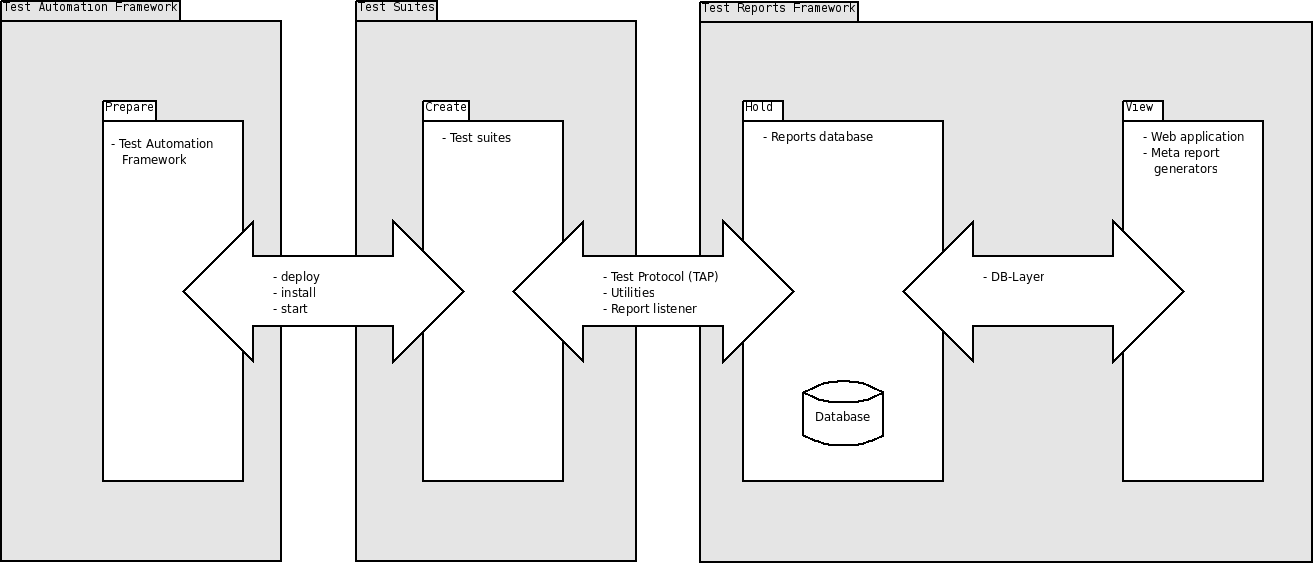
\includegraphics[scale=0.25]{img/tapper_architecture_overview.png}
	\end{center}
	\caption{Overview of the \tapper architecture}
	\label{fig:architecture}
\end{figure}

The components of the \releasetesting~Framework are listed in Table~\ref{tbl:components}. 

\begin{table}
  \begin{center}

    \begin{tabularx}{\linewidth}{l|X}
      {\bf\centering \releasetesting component name} & {\bf\centering Description} \\\hline
%        \texttt{Agent} & Communicates with service insances and requests a job to execute. Upon receiving the job downloads the input 
%                         files, executes the job, uploads job output files and reports that the job execution is finished. \\
%        \texttt{Generic Job and Storage Manager} & Distributes jobs from the internal queue to Agents for execution, provides space for storing 
%                                                   the job output   \\
%        \texttt{AliEn Job Manager} & Retrieves jobs from the central task queue of \indexed{AliEn} Grid \cite{alien} and sends them to 
%                                     Agents for execution \\
%        \texttt{AliEn Storage Manager} & Uploads the output of AliEn jobs executed by Agents and finalizes the job status in AliEn Grid.  \\
%        \texttt{PanDA Storage Manager} & Uploads the output of \indexed{PanDA} \cite{panda} jobs executed by Agents and finalizes the job status in PanDA Grid  \\
    \end{tabularx}  
  \end{center}

  \caption{List of \releasetesting and \amdtapper components}

  \label{tbl:components}
\end{table}

\chapter{\cernvmtestframework}
\section{Framework Design Overview}
\label{sec:frameworkoverview}

The \cernvmtestframework\ was initially designed to facilitate the role of ``Test Suites'' within the \releasetesting~infrastructure, which would 
execute tests and submit a report file in the form of a ``Test Anything Protocol'' (TAP) file to the ``Test Reports Framework''. This has since been
expanded to compensate for the shortcomings of \tapper and the \cernvmtestframework\ has since been expanded to comprise the role of the ``Test
Automation Framework'', which deploys, installs, and configures the \cernvm images before testing. This is important to understand as the 
``Precondition Tests'' shown in the following diagrams are mostly tests which facilitate the role of the ``Test Automation Framework'' by ensuring
that the \cernvm image host environment, and the images themselves are properly configured before executing the actual \cernvmreleasetesting test
cases.

\begin{figure}[!hbp]
	\begin{center}
		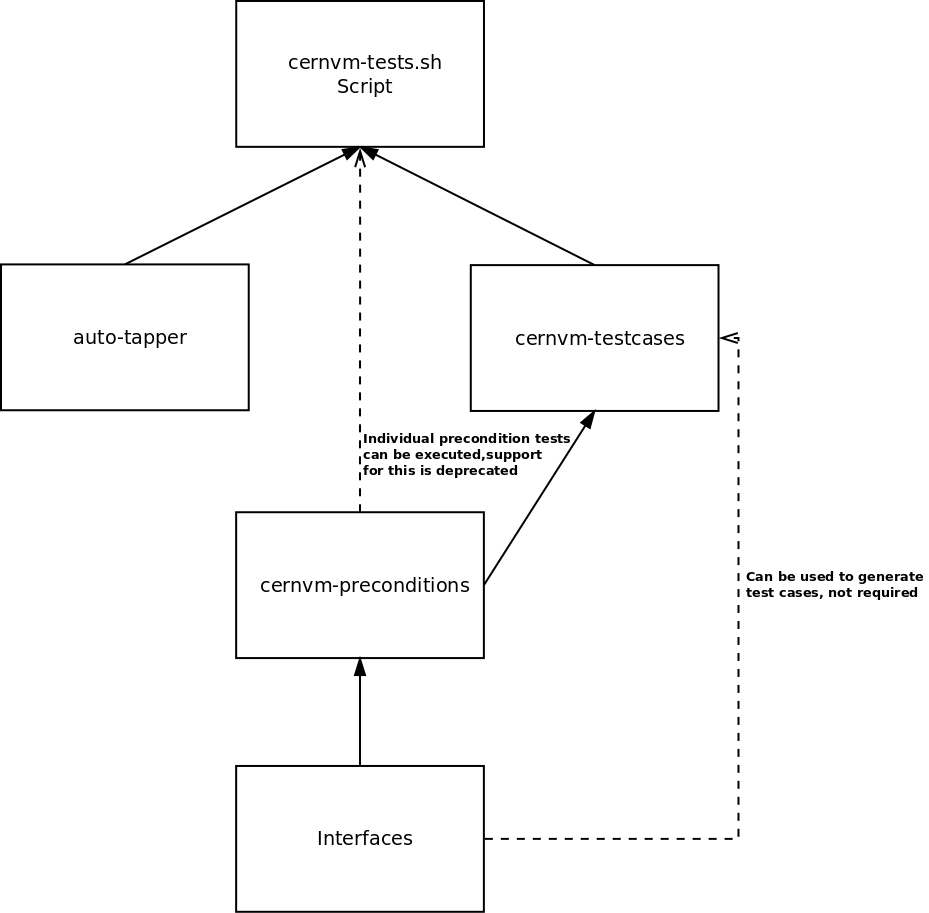
\includegraphics[scale=0.19]{img/proposed_framework.png}
	\end{center}
	\caption{Overview of the Proposed \cernvmtestframework}
	\label{fig:proposedarchitecture}
\end{figure}

\newpage
Currently, due to time constraints the optimal \cernvmtestframework\ design has not been implemented, figure~\ref{fig:proposedarchitecture} is a very
simplistic high-level overview of what the \emph{proposed} or intended final architecture is intended to be. The emphasis is on a hierarchical design
which is a result in part due to how scope is done in Bash and to limit the functions directly accessed by the {\bf cernvm-tests.sh} script to those
provided by auto-tapper and cernvm-testcases. In order for the proposed framework to be implemented, the \cernvm test cases must be modular test 
cases, independent of each other, this has not been implemented yet and as a result the following diagram outlines the current \cernvmtestframework.

\begin{figure}[hbp]
	\begin{center}
		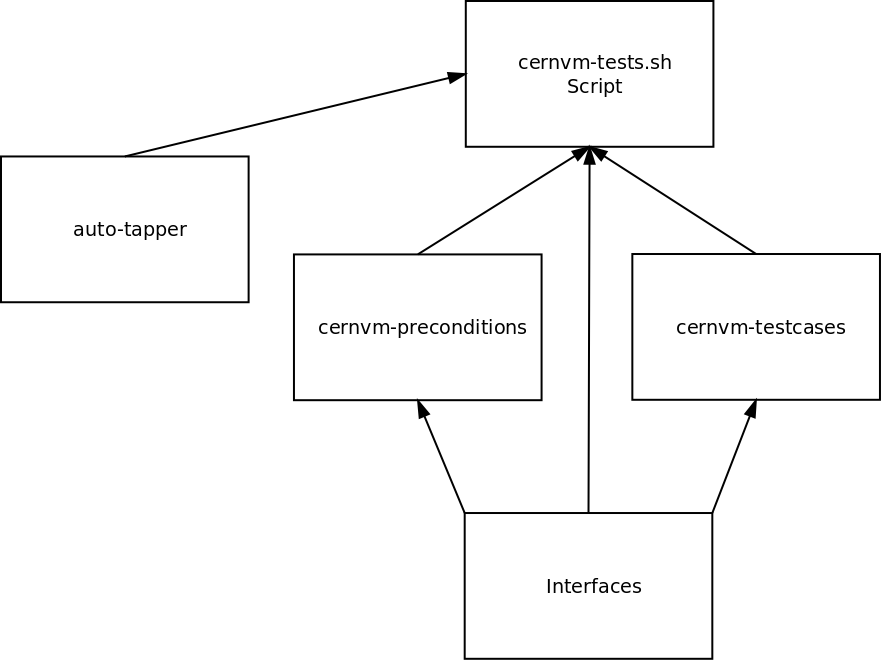
\includegraphics[scale=0.25]{img/current_framework.png}
	\end{center}
	\caption{Overview of the Current \cernvmtestframework}
	\label{fig:currentarchitecture}
\end{figure}

As shown in figure~\ref{fig:currentarchitecture} the current architecture of the \cernvmtestframework\ differs from the proposed framework because the
{\bf cernvm-tests.sh script}, \emph{which is the script that executes the set of \cernvm test cases}, requires both the {\bf cernvm-preconditions}
and {\bf cernvm-testcases} files. The {\bf cernvm-preconditions} file is what facilitates the ``Test Automation Framework'' by ensuring
that the host environment and \cernvm images are properly configured; the {\bf cernvm-testcases} file is what contains the actual
\cernvmreleasetesting test cases, which are required to test the \cernvm image. Inherently, this causes issues as there are precondition tests
that must pass before any of the test cases are executed for the results from the test cases to accurate. For example, in order to execute the test
case which verifies that the \cernvm image has SSH login support, numerous precondition tests must first be executed which create and configure the \cernvm image and verify that it can be started.

\begin{figure}[hbp]
	\begin{center}
		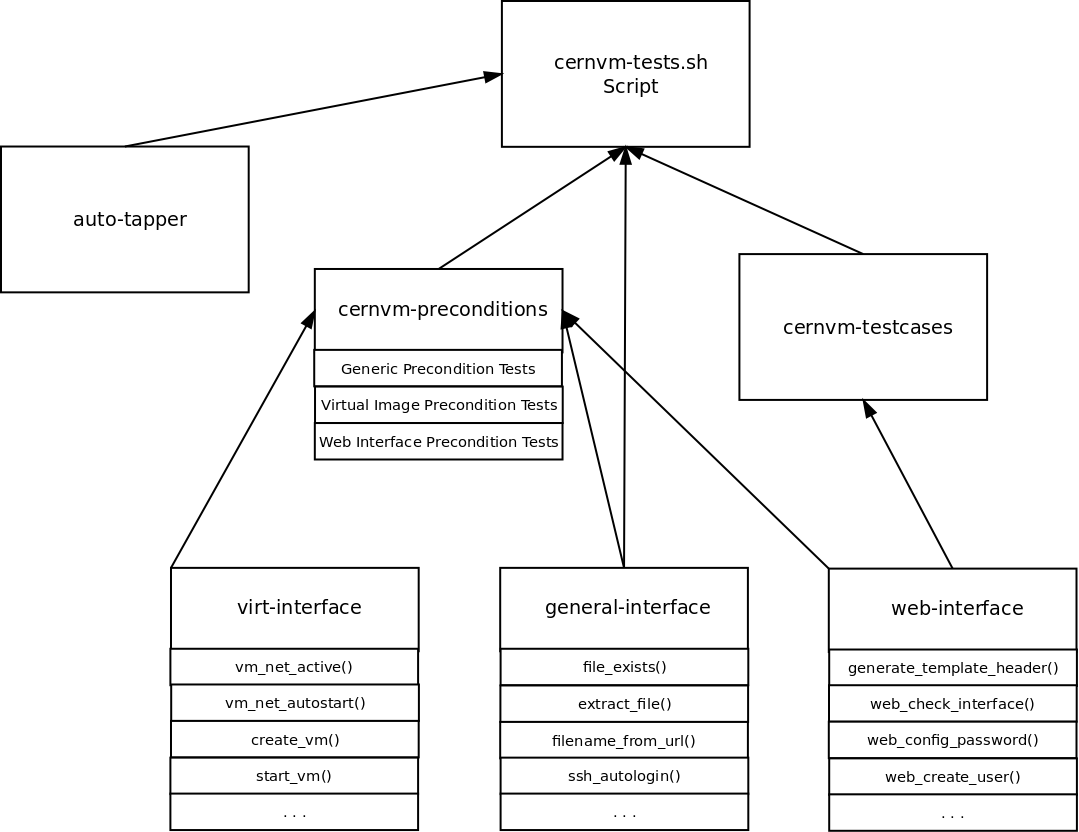
\includegraphics[scale=0.25]{img/detailed_framework.png}
	\end{center}
	\caption{Detailed Overview of the Current \cernvmtestframework}
	\label{fig:detailedarchitecture}
\end{figure}

The figure~\ref{fig:detailedarchitecture} provides a much more detailed diagram depicting the relations between the different files which are the
individual components that make up the current architecture of the \cernvmtestframework. As you can see, the hierarchy still exists to an extent
but because of the direct dependency the {\bf cernvm-tests.sh} script has on {\bf cernvm-preconditions} and {\bf cernvm-testcases} there are
precondition tests which must be executed first and in the correct order before any of the test cases can be executed.




\section{Precondition Tests}
\label{sec:preconditiontests}

Precondition tests are the tests which fulfil the role of the ``Test Automation Framework'' referred to in the \tapper architecture
figure~\ref{fig:architecture} within the \cernvmtestframework. The main purpose of the ``Precondition Tests'' is to ensure that the
host environment, and the \cernvm images themselves are properly configured before executing the actual \cernvmreleasetesting test
cases. The precondition tests configure the host environment and the \cernvm images through tests which automate deployment, 
installation, and configuration of the \cernvm images before testing.

Therefore, because the precondition tests are the tests which automate the process of setting up the host environment, the tests must
satisfied in order for a \cernvm test case to be executed accurately. In a nutshell, they are tests that must be executed, and pass before an 
actual test case can be executed. Currently, there are three categories of precondition tests, 

\begin{itemize}
\item	Generic Precondition Tests
\item	Virtual Image Precondition Tests
\item	Web Interface Precondition Tests
\end{itemize}

Generic precondition tests, as the name implies, are generic tests which provide functionality to configure the host environment and the
\cernvm image using methods that are not in the same category as the other two types of precondition tests. For example, a test that 
downloads and extracts the \cernvm image file, would be an example of a generic precondition test. Unlike generic precondition tests, 
virtual image precondition tests are very specific to configuring the virtualization environment of the \cernvm image and involve tests 
that interact with the libvirt/virsh library through the {\bf virt-interface} such as creating the virtual machine XML definition file 
and verifying the that the \cernvm image can be started. The last category of precondition tests, web interface precondition tests, 
are unique in that they are tests directly related to configuring the \cernvm image through the web interface of the \cernvm image. 
Although the web interface precondition tests could be expanded to include generic ``web'' tests, currently the precondition test are 
limited to configuring and controlling the \cernvm image through the web interface.




\section{\cernvm Test Cases}
\label{sec:cernvmtestcases}

The \cernvm Test Cases are simply the tests which fulfil the role of the ``\cernvm Test Cases'', these tests are scripted
implementations of the \cernvm Test Cases which would have otherwise been executed manually. As referred to in the
Current \cernvmtestframework\ figure~\ref{fig:detailedarchitecture}. The \cernvm Test Cases are an essential component
of the main ``cernvm-tests.sh'' script, and require both cernvm-preconditions tests as well as interface functions
to execute the test cases. The cernvm-precondition functions are essential to executing test cases as the precondition tests
are what initially set up and prepare the host environment for executing the actual test cases. In addition, the precondition
tests can be used by the \cernvm Test Cases to ensure that the minimum dependencies are met before executing the test case,
which allows for modular, or out-of-order testing. This enables a single test to be executed without having any prerequisites
for a specific precondition test or test case to have been executed before.

Therefore, the \cernvm Test Cases differ fom precondition tests because they are merely tests which automate the otherwise
manual process of executing the test cases and checking the \cernvm image. Unlike precondition tests, test cases are not required to
pass in order for another \cernvm test case to be executed accurately, any dependencies required for a test case to execute
accurately should be instead satisfied by a precondition test. Thus, the results of a test case should not have any
influence on the results of another test case, unless they are part of an actual test dependency, any test case requirements
such as having network support, or the virtual machine started and configured should be executed by precondition tests.
\chapter{Test Suite Configuration File}
\label{sct:configfile}

The configuration file is essential to setting up the initial \cernvm test suite for testing, while most of the default 
settings provided in the configuration file are sufficient for most \cernvm image testing environments, there are still
some mandatory settings which {\bf must be configured before testing can begin}. In addition to the mandatory settings
that must be specified before tests can be executed, there are also optional configuration settings which provide settings
that can override the default settings normally taken when the default configuration file is used, these include options
to override the default virtual machine settings specified in the template files.

Each group of settings has a unique prefix depending on the category of setting, there are four categories of options
for both the mandatory and optional settings that can be provided. The four setting prefixes are {\bf TS, VM, WEB, TC}
these denote options that are specific to a category of configuration options. The following is brief summary of each
configuration setting prefix, and what category of configurations each prefix applies to.

\begin{description}
\item[{\bf TS}]		Options which have this prefix are associated with configuration settings specific to the
					\cernvmreleasetesting Test Suite

\item[{\bf VM}]		Options which have this prefix are associated with configuration settings specific to the
					\cernvm image hypervisor settings, such as the setting for the virtual machine memory
					
\item[{\bf WEB}]	Options which have this prefix are associated with configuration settings specific to the
					\cernvm web interface and configuring the virtual machine through the web interface
					
\item[{\bf TC}]		Options which have this prefix are associated with configuration settings specific to the
					\cernvm Test Cases
\end{description}


\subsection{Mandatory Settings}
\label{sct:mandatorysettings}

In most testing scenarios only the mandatory configuration settings need to be specified such as the hypervisor and 
the download page, but optional settings are also provided to override internal default settings used by the 
\cernvmtestframework\. The following is a list of the mandatory settings that must be configured in order for the
tests to work, ensure that you enter valid values, \emph{in lower-case}, for the settings indicated.




\begin{itemize}
\item	TS\_SUITENAME
		\begin{itemize}
		\item	Must ALWAYS be set, only define once at the top of the configuration file, 
	  		  	usually the default suite name given in the test suite configuration file is fine
		\end{itemize}
	  		  
\item	TS\_SUITEVERSION
		\begin{itemize}
		\item	Must ALWAYS be set, only define once at the top of the configuration file,
	  		  	reflects the release version number of the test suite framework, the default 
      		  	suite version given in the test suite configuration should only be changed if 
     		  	you make modifications to the test suite framework which differentiate it from
      		  	the version released on Google Code.
		\end{itemize}

\item	TS\_REPORT\_SERVER
		\begin{itemize}
		\item	Must ALWAYS be set, only define once at the top of the configuration file,
      			this is the ip address or hostname of the Tapper report server which the reports
      			from the test results are sent to
		\end{itemize}
		
\item	TS\_DOWNLOAD\_PAGE
		\begin{itemize}
		\item	Must ALWAYS be set, normally the default url provided in the configuration file is
				accurate, but in the event that the internal \cernvm image release page is relocated
				then this url must be changed.
		\end{itemize}

\item	VM\_HYPERVISOR
		\begin{itemize}
		\item	Must ALWAYS be set, MUST be the first setting before the rest of the mandatory
	  			and optional settings specific to the hypervisor are set
	  	\item	Valid values (case sensitive) are {\bf kvm,vbox,vmware}
		\end{itemize}

\item	VM\_TEMPLATE
		\begin{itemize}
		\item	Must ALWAYS be set, normally the default template provided in the configuration file
				should not be changed, only change this to use a custom template file for the \cernvm 
				image
		\item	The custom template file \emph{must be placed within the templates folder}
		\end{itemize}

\item	VM\_NET\_TEMPLATE
		\begin{itemize}
		\item	Must ALWAYS be set, normally the default network template provided in the configuration file
				should not be changed, only change this to use a custom network template file for the \cernvm 
				image
		\item	The custom network template file \emph{must be placed within the templates folder}
		\item 	The network template file, {\bf only applies to kvm and virtualbox}
		\end{itemize}

\item	VM\_IMAGE\_VERSION
		\begin{itemize}
		\item	Must ALWAYS be set,  MUST be defined for the HYPERVISOR entry in the configuration
				file, specifies the version of the CernVM image to use from the release page
		\end{itemize}
	
\item	VM\_IMAGE\_TYPE
		\begin{itemize}
		\item	Must ALWAYS be set,  MUST be defined for the HYPERVISOR entry in the configuration
				file, specifies the type of CernVM image, such as desktop, basic, head node, etc
		\item	Valid image types supported, (case sensitive) are {\bf basic and desktop}
		\end{itemize}
		
\item	VM\_ARCH
		\begin{itemize}
		\item	Must ALWAYS be set, MUST be defined for the HYPERVISOR entry in the configuration
				file, specifies the architecture of the \cernvm image
		\item	Valid architectures (case sensitive) are {\bf x86 and x86\_64}
		\end{itemize}

% perhaps make these optional...
%export VM_TEMPLATE="cernvm-vbox.xml"
%export VM_NET_TEMPLATE="vbox-network.xml"
%export VM_IMAGE_VERSION="2.4.0"		

\end{itemize}




\subsection{Optional Settings}
\label{sct:optionalsettings}

In most testing scenarios only the mandatory configuration settings need to be specified such as the hypervisor and 
the download page, but optional settings are also provided to override internal default settings used by the 
\cernvmtestframework\. The following is a list of the optional settings that may be specified to override the default
settings, the optional settings must be configured for each of the HYPERVISOR settings defined in the configuration file.
The optional settings are separated primarily into four categories, host settings, virtual machine settings, web interface
settings, and test case settings. 

Again, only the mandatory settings are required to be specified in order for the tests to work, the optional settings 
can be ignored completely and the test suite scripts should still execute correctly. Therefore, optional settings should
only be specified by advanced users as improper optional settings can cause precondition tests to return failures,
\emph{it is only recommended that you start configuring optional settings after verifying the results of the scripts 
using only the mandatory settings}.


\paragraph*{Optional Host Settings}
\begin{itemize}
\item	TS\_IMAGES\_DIR
		\begin{itemize}
		\item	The root directory for the location of the \cernvm images and all
				configuration files and settings, by default /usr/share/images on
				Linux/OS X systems and \verb|C:\users\default\application data\images|
				on Windows systems
		\end{itemize}
		
\item	TS\_OSNAME
		\begin{itemize}
		\item	The name of the host operating system, such as Red Hat 5, OS X
				Snow Leopard, or Windows 7, configure accordingly
		\item	\emph{Support may be added eventually to automatically configure OSNAME}
		\end{itemize}
		
\item	TS\_HOSTNAME
		\begin{itemize}
		\item	The hostname of the system, determined automatically by the script,
				only set this if you wish to override the default hostname of the
				system
		\end{itemize}
\end{itemize}


\paragraph*{Optional Virtual Machine Settings}~\newline

The following are the optional virtual machine settings which can be specified to override
the default settings used by the \cernvmtestframework\, these default virtual machine settings
used by the framework are based on the virtual machine XML template definition files defined
in the templates directory.
 
\begin{itemize}
\item	VM\_NAME
		\begin{itemize}
		\item	Overrides the default name of the virtual machine set by the 
				virtual machine template XML defintion file
		\item	It is recommended that this setting is specified if testing multiple
				versions of the same \cernvm image, for example a name such as
				``cernvm-vbox-2.4.0'' would help differentiate between other versions
		\end{itemize}
		
\item	VM\_CPUS
		\begin{itemize}
		\item	Overrides the default number of cpus, which is one cpu by default,
				set by the virtual machine template XML defintion file
		\item	Valid values are from {\bf 1 - 4}, but the number specified cannot
				exceed the actual number of cores/cpus on the host system
		\end{itemize}
	
\item	VM\_MEMORY
		\begin{itemize}
		\item	Overrides the default default amount of memory set by the virtual machine
				template XML defintion file
		\item	It is recommended that you specify this value if thrashing occurs on the
				\cernvm image when executing tests due to a lack of memory
		\item	Valid values are in kilobytes and must be based on an amount of memory in
				kilobytes that is a multiple of a base value of 2. For example, to increase
				the memory of a system to 1024 MB, set the value as {\bf 1048576}, which is the
				amount of memory in kilobytes
		\end{itemize}
		
\item	VM\_VIDEO\_MEMORY
		\begin{itemize}
		\item	Overrides the default amount of video memory set by the virtual machine
				template XML defintion file
		\item	It is recommended that you specify this value if display errors occurs on the
				\cernvm image before or when executing tests due to a lack of video memory
		\item	Valid values are in kilobytes and must be based on an amount of video memory in
				kilobytes that is a multiple of a base value of 2. For example, to increase
				the video memory of a system to 64 MB, set the value as {\bf 65536}, which is the
				amount of video memory in kilobytes
		\end{itemize}
		
\item	VM\_NET\_NAME
		\begin{itemize}
		\item	Overrides the default virtual network name set by the virtual machine
				template XML defintion file
		\item	This is the one optional setting {\bf you should never configure}, unless you have
	  			manually created a different virtual network for the hypervisor
		\end{itemize}


\end{itemize}


\paragraph*{Optional Web Interface Settings}~\newline

The following are the optional web interface settings which can be specified to override
the default settings used by the \cernvmtestframework\, such as the \cernvm image desktop
resolution and the primary experiment group.

\begin{itemize}
\item	WEB\_ADMIN\_USERNAME
		\begin{itemize}
		\item	Overrides the default web inteface administration account user name,
				which is ``admin'' by default. This optional settings should not 
				have to be modified unless the \cernvm web interface defaults change
		\end{itemize}
		
\item	WEB\_ADMIN\_DEFAULT\_PASS
		\begin{itemize}
		\item	Overrides the default web interface administration account password,
				which is ``password'' by default. This optional settings should not 
				have to be modified unless the \cernvm web interface defaults change
		\end{itemize}
		
\item	WEB\_ADMIN\_PASS
		\begin{itemize}
		\item	Overrides the web inteface administration account password set by
				the test suite scripts with a user defined web interface
				administration password
		\item	The password specified {\bf must be six characters or longer}
		\end{itemize}

\item	WEB\_USER\_NAME
		\begin{itemize}
		\item	Overrides the default account name ``alice'' of the new user created 
				by the test suite scripts through the web interface
		\item	The user name specified should only contain alphabetical characters
		\end{itemize}
		
\item	WEB\_USER\_PASS
		\begin{itemize}
		\item	Overrides the default password ``VM4l1f3'' of the new user created 
				by the test suite scripts through the web interface
		\item	The password specified {\bf must be six characters or longer}
		\end{itemize}

%TODO ADD A LIST OF THE VALID GROUPS FOR THE NEW USER
\item	WEB\_USER\_GROUP
		\begin{itemize}
		\item	Overrides the default group ``alice'' for the new user created 
				by the test suite scripts through the web interface
		\item	The group specified must be a valid group available
				through the web interface, such as ``alice''
		\end{itemize}

\item	WEB\_ROOT\_PASS
		\begin{itemize}
		\item	Overrides the default password ``VM4l1f3'' of the root account
				on the \cernvm image set by the test suite scripts through the
				web interface
		\item	The password specified {\bf must be six characters or longer}
		\end{itemize}
		
\item	WEB\_STARTXONBOOT
		\begin{itemize}
		\item	Overrides the default \cernvm desktop setting set by the test 
				suite scripts through the web interface, which configures X to
				start on boot
		\item	The valid values, (lower-case) are either ``on'' to start X on boot,
				\emph{which is the default}, or ``off'' to not start X on boot		
		\end{itemize}
				
%TODO GET A LIST OF THE VALID RESOLUTIONS ACCEPTED BY THE WEB INTERFACE
\item	WEB\_RESOLUTION
		\begin{itemize}
		\item	Overrides the default \cernvm desktop resolution, {\bf 1024x768} set by
				the test suite scripts through the web interface
		\item	The valid values are valid resolutions up to a {\bf maximum resolution
				of 1680x1050}
		\end{itemize}

%TODO GET A LIST OF THE VALID KEYBOARD LOCALES
\item	WEB\_KEYBOARD\_LOCALE
		\begin{itemize}
		\item	Overrides the default \cernvm desktop keyboard locale, which is ``us'' by
				default, set by the test suite scripts through the web interface
		\item	The valid values are valid locale settings
		\end{itemize}

\item	WEB\_EXPERIMENT\_GROUP
		\begin{itemize}
		\item	Overrides the default \cernvm primary experiment group, which is ``ALICE''
				by default, set by the test suite scripts through the web interface
		\item	The valid values are one of following group names, {\bf the group name
				specified must be in UPPERCASE}: ALICE, ATLAS, CMS, LHCB, LCD, NA61, HONE,
				HEPSOFT, BOSS, GEANT4	
		\end{itemize}
\end{itemize}


\paragraph*{Optional Test Case Settings}~\newline

The following are the optional test case settings which can be specified to override
the default settings used by the \cernvmtestframework\ for executing the \cernvmreleasetesting
test cases.

\begin{itemize}
\item	TC\_USER\_NAME
		\begin{itemize}
		\item	Overrides the default account name ``bob'' of the new user created 
				through the web interface as part of a \cernvmreleasetesting test case
		\item	The user name specified should only contain alphabetical characters
		\end{itemize}
		
\item	TC\_USER\_PASS
		\begin{itemize}
		\item	Overrides the default password ``R00tM3'' of the new user created 
				through the web interface as part of a \cernvmreleasetesting test case
		\item	The password specified {\bf must be six characters or longer}
		\end{itemize}
\end{itemize}
\chapter{Adding \cernvm Test Cases}
\section{Adding Test Cases Overview}
\label{sec:addtestsoverview}

The \cernvm Test Cases are simply the tests which fulfil the role of the ``\cernvm Test Cases'', these tests are just scripted
implementations of the \cernvm Test Cases which would have otherwise been executed manually. The \cernvm Test Cases
are an essential component of the main ``cernvm-tests.sh'' script and require both cernvm-preconditions tests as well as
interface functions to execute the test cases. The cernvm-precondition functions are essential to executing test cases as the 
precondition tests are what initially set up and prepare the host environment for executing the actual test cases. In addition,
the precondition tests can be used by the \cernvm Test Cases to ensure that the minimum dependencies are met before
executing the test case, which allows for modular, or out-of-order testing. This enables a single test to be executed without
having any prerequisites for a specific precondition test or test case to have been executed before.

Therefore, the \cernvm Test Cases differ fom precondition tests because they are merely tests which automate the otherwise
manual process of executing the test cases and checking the \cernvm image. Unlike precondition tests, test cases are not required to
pass in order for another \cernvm test case to be executed accurately, any dependencies required for a test case to execute
accurately should be instead satisfied by a precondition test. 

Thus, unlike precondition tests, the test cases should only contain the functionality essential to executing the \cernvm Test Cases,
anything that could be seen as a prerequisite to executing a test case, such as starting or restarting a virtual machine should
not be part of the test case code. \emph{This is important as separating prerequisites from actual test cases enables modular,
or out of order testing}; writing prerequisites to test cases as precondition tests allows a single test to be executed independently
or the results or execution of another test case.


\section{Example, Adding a New Test Case}
\label{sec:addnewtest}

The following will be an example of adding a \cernvm Test Case which verifies that it is possible to login to the \cernvm image
using SSH, there will be code samples provided, as well as a detailed explanation of the entire procedure to add a new test case
and intergrate it with the ``cernvm-tests.sh'' script.

\begin{enumerate}

\item	The first step to take before adding a single line of code is to sit down and analyze any prerequisites for executing the
			test case, any condition that must be met before the actual test case can be executed can be considered a prerequisite
			and thus would be a precondition test.  First start by creating a list of any procedures that would have to be manually
			executed before actually executing the test case, such as starting the virtual machine and verifying that it has network
			access.
			
			For the test case used in this example, which verifies that it is possible to login to the \cernvm image using SSH, the
			list of prerequisites could be listed as something similar to the following.
			
			\begin{itemize}
			\item	Download and extract the \cernvm image
			\item	Create the virtual machine
			\item	Configure the virtual machine for testing, such as the amount of memory
			\item	Start the virtual machine
			\item	Configure the \cernvm image through the web interface, add a new user, configure experiment group
			\end{itemize}
			
\item	Next, refer to the API reference for a comprehensive list of the precondition tests and interface functions  available 
			and look for any precondition tests or functions that satisfy the prerequisites needed to execute the test case. Specifically,
			refer to the section titled, ``test-suite/cernvm-preconditions''~\ref{ch:test_suite_cernvm_preconditions}, which has every 
			precondition test function documented, including a description of what the precondition test does and the arguments and
			return values.
			
			For the test case used in this example, all of the prerequisites listed in the previous step can be executed
			by existing precondition tests and interface functions. Thus, there is a high probability that many of the prerequisites for
			each test case have been already satisfied by a precondition test. The following is a list of the precondition tests and
			interface functions that satisfy all of the prerequisites listed in the previous step.
			
			\begin{itemize}
				\item	download\_extract()
				\item	create\_def()
				\item	verify\_hypervisor()
				\item	create\_vm()
				\item	start\_vm()
				\item	web\_check\_interface()
				\item	web\_check\_login()
				\item	configure\_image\_web()
			\end{itemize}
			
\item	Now that the functions necessary to meet all of the prerequisites for the \cernvm test case have been determined, the next
			step involves determining the variables and values to pass to the precondition tests and other interface functions. After determining 
			the arguments to the functions, determine which configuration options should be specified in the configuration file to be passed as
			arguments to the functions, as almost all of the variables required by the functions should be specified in the configuration file and
			not set in the cernvm-tests.sh script itself. For a complete list of the available configuration options refer to section~\ref{sec:configfile},
			remember that it is not essential to specify every optional configuration setting as all of the configuration options which are not mandatory 
			have default values.
			
			For the test case used in this is example the KVM \cernvm image will be used to verify SSH access, therefore only the two
			mandatory configuration options ``CVM\_TS\_REPORT\_SERVER'' and ``CVM\_VM\_IMAGE\_VERSION'' would have to 
			be specified in the provided kvm configuration file \verb|content/cernvm-kvm.cfg|. This is because all of the arguments
			required by the functions listed in the previous step have suitable default values specified in the cernvm-tests.sh script
			if the optional configuration setting is not specified. For example, the following code snippet from \emph{cernvm-tests.sh}
			demonstrates the suiteable default values for the variables required by the configure\_image\_web() function, which
			configures the \cernvm image through the web interface.
			
\lstset{language=bash,caption=Suiteable Default Values for the Web Interface}
\begin{lstlisting}
######### Optional Web Interface Settings ##########
ADMIN_USERNAME="${CVM_WEB_ADMIN_USERNAME:-admin}"
ADMIN_DEFAULT_PASS="${CVM_WEB_ADMIN_DEFAULT_PASS:-password}"
ADMIN_PASS="${CVM_WEB_ADMIN_PASS:-VM4l1f3}"

# CernVM image user settings, specify the settings for new account
USER_NAME="${CVM_WEB_USER_NAME:-alice}"
USER_PASS="${CVM_WEB_USER_PASS:-VM4l1f3}"
USER_GROUP="${CVM_WEB_USER_GROUP:-alice}"

# CernVM image root account settings, specify password for root account
ROOT_PASS="${CVM_WEB_ROOT_PASS:-VM4l1f3}"

# CernVM image desktop settings
STARTXONBOOT="${CVM_WEB_STARTXONBOOT:-on}"
RESOLUTION="${CVM_WEB_RESOLUTION:-1024x768}"
KEYBOARD_LOCALE="${CVM_WEB_KEYBOARD_LOCALE:-us}"

# CernVM image primary group (experiment) settings
EXPERIMENT_GROUP="${CVM_WEB_EXPERIMENT_GROUP:-ALICE}"
\end{lstlisting}
			
\item	Now that the functions, variables, and configuration options necessary to meet all of the prerequisites for 
			the \cernvm test cases have been determined. The next step involves adding the precondition tests and 
			other interface functions to the main ``cernvm-tests.sh'' script in a form that can be handled by 
			tapper-autoreport. While the cernvm-tests.sh script is simply a script that has an incremental list of the 
			precondition tests and test cases to be executed, the precondition tests and test cases still need to be
			integrated with tapper-autoreport so that the results of the tests can be added to the Test Anything Protocol
			(TAP) report, which is submitted to the \tapper Server.
			
			Because many of the test cases share similar prerequisites, such as the virtual machine first being created and
			started, it is best to place the ordered list of precondition tests within the cervnvm-tests.sh script before calling
			the test case function. By placing the calls to precondition tests directly in the cernvm-tests.sh script instead
			of calling them from a test case function, test case dependencies can be avoided as the prerequisites for most
			of the \cernvm test cases are met before any test case functions are called.
			
\item	After adding the ordered list of precondition tests to the cernvm-tests.sh script, the next step is to integrate
			the precondition tests with tapper-autoreport so that the results of the tests can be added to the Test Anything 
			Protocol (TAP) report and submitted to the \tapper Server. The easiest method of doing this is to catch the exit
			status of the functions called, which is provided internally by bash using the variable {\bf \$?} and pass the exit
			status to the tapper-autoreport function {\bf ok}. The tapper-autoreport function, {\bf ``ok''} takes two arguments,
			the return code and report message; the most practical method of specifying the report message is to use
			the precondition test's function description from the API reference and use an incremental counter for each test.
			
			The following code snippet from \emph{cernvm-tests.sh} is an example of implementing the precondition tests
			before calling any test case functions and integrating the results of the precondition tests with the auto-tapper
			reporting facilities. All of the variables used in the function calls are either set based on the options provided in
			the configuration file or use default values if the optional configuration options are not specified.

\lstset{language=bash,caption=Adding Precondition Tests and Integrating with Tapper-AutoReport}
\begin{lstlisting}

######### Optional CernVM Image Settings ##########
IMAGE_RELEASE_ID="${CVM_VM_IMAGE_RELEASE_ID}"
NAME="${CVM_VM_NAME:-cernvm-${HYPERVISOR}-${IMAGE_VERSION}}"

######### Optional Web Interface Settings ##########
ADMIN_USERNAME="${CVM_WEB_ADMIN_USERNAME:-admin}"
ADMIN_DEFAULT_PASS="${CVM_WEB_ADMIN_DEFAULT_PASS:-password}"
ADMIN_PASS="${CVM_WEB_ADMIN_PASS:-VM4l1f3}"

######### CernVM Image Settings ##########
VM_XML_DEFINITION="" # Leave blank, the virtual machine definition file

. . .

# Precondition Test 14 - Verify that virtual machine can be started
start_vm ${VM_XML_DEFINITION} $NAME
ok $? "Precondition Test 14 - Verify that virtual machine $VMNAME \
has been started"

. . .

# Precondition Test 17 - Verify that virtual machine has web interface
#                                     support
web_check_interface ${IP_ADDRESS} web_interface.log
ok $? "Precondition Test 17 - Verify that virtual machine $VMNAME has web \
interface support"


# Precondition Test 18 - Verify that it is possible to login on
#                                     web interface
web_check_login ${IP_ADDRESS} $ADMIN_USERNAME $ADMIN_DEFAULT_PASS \
web_interface_login.log
ok $? "Precondition Test 18 - Verify that it is possible to login on\
web interface"


# Precondition Test 19 - Setup and configure the initial CernVM image 
#                                     through the web interface
configure_image_web ${IP_ADDRESS} $ADMIN_USERNAME $ADMIN_DEFAULT_PASS \
web_config_image.log
ok $? "Precondition Test 19 - Setup and configure the initial CernVM image \
through the web interface"
\end{lstlisting}

\item	Finally, the last step involves adding the new test case manually, again review the API reference~\ref{ch:robo32}
			and look for any functions that may already provide the necessary functionality for the test case. In the event that
			the functionality needed has not already been implemented, create new functions in one of the appropriate interface
			files. Then, implement a function for the new test case in the ``cernvm-testscases'' file and call the test case function
			from ``cernvm-tests.sh'' and integrate the results with tapper-autoreport.
						
			In some cases, there is a precondition test which already provides the functionality needed to implement the test case
			and simply needs to be called with arguments specific to the test case. This is the scenario for the test case used
			in this example, a precondition test already exists to verify that the root account has SSH access, to  create the new
			test case the arguments for the precondition test simply need to be changed.

\lstset{language=bash,caption=Adding a New Test Case and Integrating with Tapper-AutoReport}
\begin{lstlisting}

### To implement the test case call the existing precondition test 
### and verify that a specific user, instead of the default root
### account has SSH access
			 
# Add the test case function to cernvm-tests.sh that verifies SSH access
check_ssh()
{
    verify_ssh_login $1 $2

    return $?
}

### Finally add the test case to cernvm-tests.sh and 
### Integrate the results of function with tapper-autoreport

# CernVM Test Case 1 - Check login via ssh as user created through
#                                    the web interface
check_ssh ${IP_ADDRESS} $USER_NAME
ok $? "CernVM Test Case 1 - Check login via ssh as user created \
through web interface"
\end{lstlisting}
			

\end{enumerate}


% For now, directly include the api reference generated by ROBODoc
\chapter{Test Suite API Reference}
\label{sct:apireference}
% Document: ./content/apireference
% Source: ./../../tapper/tapper-autoreport/
% Generated with ROBODoc Version 4.99.41 (Oct  2 2011)
\newpage
\section{test-suite/cernvm-preconditions}
\textsl{[ Generics ]}

\label{ch:robo40}
\label{ch:test_suite_cernvm_preconditions}
\index{unsorted!cernvm-preconditions}\index{Generics!cernvm-preconditions}
\textbf{NAME}
\begin{verbatim}
   cernvm-preconditions
\end{verbatim}
\textbf{DESCRIPTION}
\begin{verbatim}
   This script contains each of the CernVM Release Testing precondition
   tests, which are required preconditions that must pass for the results 
   of test cases to be accurate. The precondition tests have a simple
   interface to execute each test and each test returns either a success or 
   failure, (0 or 1)

   More complex precondition tests can be created by combining other 
   precondition tests as prerequisites for a precondition test
\end{verbatim}
\textbf{TODO}
\begin{verbatim}
   CLEAN UP THE FOLLOWING PRECONDITON TESTS AND PLACE THEM IN THIS FILE
   Precondition Test 2 - Verify that virtual machine domain has been created 
                         from an xml file

   Precondition Test 3 - Verify that virtual machine can be started

   Precondition Test 4 - Verify that virtual machine has been stopped

   Precondition Test 5 - Verify that the virtual has console support

   Precondition Test 6 - Verify that virtual machine has web interface support

   Precondition Test 7 - Verify that it is possible to login on web interface
\end{verbatim}
\newpage
\subsection{cernvm-preconditions/configure\_image\_web}
\textsl{[ cernvm-preconditions ]}
\textsl{[ Functions ]}

\label{ch:robo0}
\label{ch:cernvm_preconditions_configure_image_web}
\index{unsorted!configure\_image\_web}\index{Functions!configure\_image\_web}
\textbf{NAME}
\begin{verbatim}
   configure_image_web
\end{verbatim}
\textbf{DESCRIPTION}
\begin{verbatim}
   Precondition Test - Setup and configure the initial CernVM image through the
   web interface
\end{verbatim}
\textbf{ARGUMENTS}
\begin{verbatim}
   $1 - The hostname or ip address for the web interface
   $2 - The default username to access web interface
   $3 - The default password to access web interface
\end{verbatim}
\textbf{RESULT}
\begin{verbatim}
   exitstatus - Sets $? as a zero for success, otherwise sets an error code
\end{verbatim}
\textbf{EXAMPLE}
\begin{verbatim}
   configure_image_web 192.168.1.125 admin password config-image.log
\end{verbatim}
\textbf{TODO}
\begin{verbatim}
   Implement a function that uses curl to get the updates from the web server 
   to determine when the system has rebooted
\end{verbatim}
\newpage
\subsection{cernvm-preconditions/create\_def}
\textsl{[ cernvm-preconditions ]}
\textsl{[ Functions ]}

\label{ch:robo1}
\label{ch:cernvm_preconditions_create_def}
\index{unsorted!create\_def}\index{Functions!create\_def}
\textbf{NAME}
\begin{verbatim}
   create_def
\end{verbatim}
\textbf{DESCRIPTION}
\begin{verbatim}
   Precondition Test - Create an XML definition file for the virtual machine based
   on the template XML definition file and settings defined and return the
   location of the xml defintion file created
\end{verbatim}
\textbf{ARGUMENTS}
\begin{verbatim}
   $1 - The template file to use
   $2 - The directory to save the final xml definition file in
\end{verbatim}
\textbf{RETURN VALUE}
\begin{verbatim}
   definitionfile - The location of the xml defintion file created
\end{verbatim}
\textbf{RESULT}
\begin{verbatim}
   exitstatus - Sets $? as a zero for success, otherwise sets an error code
\end{verbatim}
\textbf{EXAMPLE}
\begin{verbatim}
   create_def vm-template.xml /root
\end{verbatim}
\newpage
\subsection{cernvm-preconditions/create\_net}
\textsl{[ cernvm-preconditions ]}
\textsl{[ Functions ]}

\label{ch:robo2}
\label{ch:cernvm_preconditions_create_net}
\index{unsorted!create\_net}\index{Functions!create\_net}
\textbf{NAME}
\begin{verbatim}
   create_net
\end{verbatim}
\textbf{DESCRIPTION}
\begin{verbatim}
   Precondition Test - Verify that the virtual machine network has been created 
   from an xml file
\end{verbatim}
\textbf{ARGUMENTS}
\begin{verbatim}
   $1 - The path to the network XML definition file
   $2 - The virtual machine network name 
\end{verbatim}
\textbf{RESULT}
\begin{verbatim}
   exitstatus - Sets $? as a zero for success, otherwise sets an error code
\end{verbatim}
\textbf{EXAMPLE}
\begin{verbatim}
   create_net ./network-definition.xml default
\end{verbatim}
\newpage
\subsection{cernvm-preconditions/create\_net\_def}
\textsl{[ cernvm-preconditions ]}
\textsl{[ Functions ]}

\label{ch:robo3}
\label{ch:cernvm_preconditions_create_net_def}
\index{unsorted!create\_net\_def}\index{Functions!create\_net\_def}
\textbf{NAME}
\begin{verbatim}
   create_net_def
\end{verbatim}
\textbf{DESCRIPTION}
\begin{verbatim}
   Precondition Test - Create an XML definition file for the virtual machine network
   based on the template network XML definition file and settings defined and 
   return the location of the created xml defintion file
\end{verbatim}
\textbf{ARGUMENTS}
\begin{verbatim}
   $1 - The network template file to use
   $2 - The directory to save the final network xml definition file in
\end{verbatim}
\textbf{RETURN VALUE}
\begin{verbatim}
   netdefinitionfile - The location of the network xml defintion file created
\end{verbatim}
\textbf{RESULT}
\begin{verbatim}
   exitstatus - Sets $? as a zero for success, otherwise sets an error code
\end{verbatim}
\textbf{EXAMPLE}
\begin{verbatim}
   create_net_def network-template.xml /root
\end{verbatim}
\newpage
\subsection{cernvm-preconditions/download\_extract}
\textsl{[ cernvm-preconditions ]}
\textsl{[ Functions ]}

\label{ch:robo4}
\label{ch:cernvm_preconditions_download_extract}
\index{unsorted!download\_extract}\index{Functions!download\_extract}
\textbf{NAME}
\begin{verbatim}
   download_extract
\end{verbatim}
\textbf{DESCRIPTION}
\begin{verbatim}
   Precondition Test - Download and extract the CernVM image, returns the location 
   of the extracted cernvm image file
\end{verbatim}
\textbf{ARGUMENTS}
\begin{verbatim}
   $1 - The CernVM image download url
   $2 - The directory to place the downloaded image in
   $3 - The name of the log file
\end{verbatim}
\textbf{RETURN VALUE}
\begin{verbatim}
   imagelocation - The location of the extracted CernVM image file
\end{verbatim}
\textbf{RESULT}
\begin{verbatim}
   exitstatus - Sets $? as a zero for success, otherwise sets an error code
\end{verbatim}
\textbf{EXAMPLE}
\begin{verbatim}
   IMAGE_LOCATION=$(download_extract http://someurl/file.vmdk.gz /root dl-extract.log)
\end{verbatim}
\newpage
\subsection{cernvm-preconditions/image\_url}
\textsl{[ cernvm-preconditions ]}
\textsl{[ Functions ]}

\label{ch:robo5}
\label{ch:cernvm_preconditions_image_url}
\index{unsorted!image\_url}\index{Functions!image\_url}
\textbf{NAME}
\begin{verbatim}
   image_url
\end{verbatim}
\textbf{DESCRIPTION}
\begin{verbatim}
   Precondition Test - Verify that the download page exists and that there is a 
   valid download url for the CernVM image specified, returns the url to 
   download the image
\end{verbatim}
\textbf{ARGUMENTS}
\begin{verbatim}
   $1 - The CernVM download page url
   $2 - The image version
   $3 - The hypervisor of the image
   $4 - The architecture of the image
   $5 - The type of image
\end{verbatim}
\textbf{RETURN VALUE}
\begin{verbatim}
   imageurl - The url to download the image
\end{verbatim}
\textbf{RESULT}
\begin{verbatim}
   exitstatus - Sets $? as a zero for success, otherwise sets an error code
\end{verbatim}
\textbf{EXAMPLE}
\begin{verbatim}
   IMAGE_URL=$(image_url http://downloadpage.com 2.4.0 kvm x86 desktop)
\end{verbatim}
\newpage
\subsection{cernvm-preconditions/validate\_def\_settings}
\textsl{[ cernvm-preconditions ]}
\textsl{[ Functions ]}

\label{ch:robo6}
\label{ch:cernvm_preconditions_validate_def_settings}
\index{unsorted!validate\_def\_settings}\index{Functions!validate\_def\_settings}
\textbf{NAME}
\begin{verbatim}
   validate_def_settings
\end{verbatim}
\textbf{DESCRIPTION}
\begin{verbatim}
   Precondition Test - Verify that the mandatory configuration settings for the
   virtual machine XML definition file have been provided and are valid
\end{verbatim}
\textbf{ARGUMENTS}
\begin{verbatim}
   $1 - The virtual machine XML definition file
\end{verbatim}
\textbf{RESULT}
\begin{verbatim}
   exitstatus - Sets $? as a zero for success, otherwise sets an error code
\end{verbatim}
\textbf{EXAMPLE}
\begin{verbatim}
   validate_def_settings ./vm-definition.xml
\end{verbatim}
\newpage
\subsection{cernvm-preconditions/validate\_def\_xml}
\textsl{[ cernvm-preconditions ]}
\textsl{[ Functions ]}

\label{ch:robo7}
\label{ch:cernvm_preconditions_validate_def_xml}
\index{unsorted!validate\_def\_xml}\index{Functions!validate\_def\_xml}
\textbf{NAME}
\begin{verbatim}
   validate_def_xml
\end{verbatim}
\textbf{DESCRIPTION}
\begin{verbatim}
   Precondition Test - Verify that the XML definition file provided is valid
\end{verbatim}
\textbf{ARGUMENTS}
\begin{verbatim}
   $1 - The virtual machine XML definition file
\end{verbatim}
\textbf{RESULT}
\begin{verbatim}
   exitstatus - Sets $? as a zero for success, otherwise sets an error code
\end{verbatim}
\textbf{EXAMPLE}
\begin{verbatim}
   validate_def_xml ./vm-definition.xml
\end{verbatim}
\newpage
\subsection{cernvm-preconditions/validate\_net\_settings}
\textsl{[ cernvm-preconditions ]}
\textsl{[ Functions ]}

\label{ch:robo8}
\label{ch:cernvm_preconditions_validate_net_settings}
\index{unsorted!validate\_net\_settings}\index{Functions!validate\_net\_settings}
\textbf{NAME}
\begin{verbatim}
   validate_net_settings
\end{verbatim}
\textbf{DESCRIPTION}
\begin{verbatim}
   Precondition Test - Verify that the mandatory configuration settings for the
   network XML definition file have been provided and are valid
\end{verbatim}
\textbf{ARGUMENTS}
\begin{verbatim}
   $1 - The network XML definition file
\end{verbatim}
\textbf{RESULT}
\begin{verbatim}
   exitstatus - Sets $? as a zero for success, otherwise sets an error code
\end{verbatim}
\textbf{EXAMPLE}
\begin{verbatim}
   validate_net_settings ./network-definition.xml
\end{verbatim}
\newpage
\subsection{cernvm-preconditions/verify\_autologin\_ssh}
\textsl{[ cernvm-preconditions ]}
\textsl{[ Functions ]}

\label{ch:robo9}
\label{ch:cernvm_preconditions_verify_autologin_ssh}
\index{unsorted!verify\_autologin\_ssh}\index{Functions!verify\_autologin\_ssh}
\textbf{NAME}
\begin{verbatim}
   verify_autologin_ssh
\end{verbatim}
\textbf{DESCRIPTION}
\begin{verbatim}
   Precondition Test - Enable automatic SSH login to the machine for the user
   specified using keys instead of passwords, and verify that it is possible 
   to login automatically
\end{verbatim}
\textbf{ARGUMENTS}
\begin{verbatim}
   $1 - The IP address of the machine to login via ssh
   $2 - The username to login with
   $3 - The password to login with
\end{verbatim}
\textbf{RESULT}
\begin{verbatim}
   exitstatus - Sets $? as a zero for success, otherwise sets an error code
\end{verbatim}
\textbf{EXAMPLE}
\begin{verbatim}
   verify_autologin_ssh 192.168.1.125 root password
\end{verbatim}
\textbf{TODO}
\begin{verbatim}
   Implement support to only remove the offending key line from known_hosts
   instead of deleting the entire file
\end{verbatim}
\newpage
\subsection{cernvm-preconditions/verify\_exists}
\textsl{[ cernvm-preconditions ]}
\textsl{[ Functions ]}

\label{ch:robo10}
\label{ch:cernvm_preconditions_verify_exists}
\index{unsorted!verify\_exists}\index{Functions!verify\_exists}
\textbf{NAME}
\begin{verbatim}
   verify_exists
\end{verbatim}
\textbf{DESCRIPTION}
\begin{verbatim}
   Precondition Test - Verify that a file/folder exists
\end{verbatim}
\textbf{ARGUMENTS}
\begin{verbatim}
   $1 - The location and name of the file
\end{verbatim}
\textbf{RESULT}
\begin{verbatim}
   exitstatus - Sets $? as a zero for success, otherwise sets an error code
\end{verbatim}
\textbf{EXAMPLE}
\begin{verbatim}
   verify_exists /root/file.tar.gz
\end{verbatim}
\newpage
\subsection{cernvm-preconditions/verify\_hash}
\textsl{[ cernvm-preconditions ]}
\textsl{[ Functions ]}

\label{ch:robo11}
\label{ch:cernvm_preconditions_verify_hash}
\index{unsorted!verify\_hash}\index{Functions!verify\_hash}
\textbf{NAME}
\begin{verbatim}
   verify_hash
\end{verbatim}
\textbf{DESCRIPTION}
\begin{verbatim}
   Precondition Test - Verify the hash of a file
\end{verbatim}
\textbf{ARGUMENTS}
\begin{verbatim}
   $1 - The location and name of the file
\end{verbatim}
\textbf{RESULT}
\begin{verbatim}
   exitstatus - Sets $? as a zero for success, otherwise sets an error code
\end{verbatim}
\textbf{EXAMPLE}
\begin{verbatim}
   verify_hash /root/file.tar.gz
\end{verbatim}
\textbf{TODO}
\begin{verbatim}
   Implement the verify_hash function later as it is not important at the moment
\end{verbatim}
\newpage
\subsection{cernvm-preconditions/verify\_hypervisor}
\textsl{[ cernvm-preconditions ]}
\textsl{[ Functions ]}

\label{ch:robo12}
\label{ch:cernvm_preconditions_verify_hypervisor}
\index{unsorted!verify\_hypervisor}\index{Functions!verify\_hypervisor}
\textbf{NAME}
\begin{verbatim}
   verify_hypervisor
\end{verbatim}
\textbf{DESCRIPTION}
\begin{verbatim}
   Precondition Test - Verify that the hypervisor for the current virtual machine
   tested is accessible, set the hypervisor URI as a global variable
\end{verbatim}
\textbf{ARGUMENTS}
\begin{verbatim}
   $1 - The virtual machine XML definition file
\end{verbatim}
\textbf{RETURN VALUE}
\begin{verbatim}
   URI - The current URI for the hypervisor of the virtual machine being tested
\end{verbatim}
\textbf{RESULT}
\begin{verbatim}
   exitstatus - Sets $? as a zero for success, otherwise sets an error code
\end{verbatim}
\textbf{EXAMPLE}
\begin{verbatim}
   verify_hypervisor vm-definition.xml
\end{verbatim}
\newpage
\subsection{cernvm-preconditions/verify\_ssh\_login}
\textsl{[ cernvm-preconditions ]}
\textsl{[ Functions ]}

\label{ch:robo13}
\label{ch:cernvm_preconditions_verify_ssh_login}
\index{unsorted!verify\_ssh\_login}\index{Functions!verify\_ssh\_login}
\textbf{NAME}
\begin{verbatim}
   verify_ssh_login
\end{verbatim}
\textbf{DESCRIPTION}
\begin{verbatim}
   Precondition Test - Verify that user is able to login via ssh
\end{verbatim}
\textbf{ARGUMENTS}
\begin{verbatim}
   $1 - The IP address of the machine to login via ssh
   $2 - The username to login with
\end{verbatim}
\textbf{RESULT}
\begin{verbatim}
   exitstatus - Sets $? as a zero for success, otherwise sets an error code
\end{verbatim}
\textbf{EXAMPLE}
\begin{verbatim}
   verify_ssh_login 192.168.1.125 root
\end{verbatim}
\newpage
\subsection{cernvm-preconditions/verify\_virsh\_uri}
\textsl{[ cernvm-preconditions ]}
\textsl{[ Functions ]}

\label{ch:robo14}
\label{ch:cernvm_preconditions_verify_virsh_uri}
\index{unsorted!verify\_virsh\_uri}\index{Functions!verify\_virsh\_uri}
\textbf{NAME}
\begin{verbatim}
   verify_virsh_uri
\end{verbatim}
\textbf{DESCRIPTION}
\begin{verbatim}
   Precondition Test - Verify that the URI virsh is connected to matches the
                       URI for the current hypervisor 
\end{verbatim}
\textbf{NOTES}
\begin{verbatim}
   This precondition test is useful for catching a potential libvirt or hypervisor error
   that is not caught by the scripts or virsh, for example if virsh fails to connect properly
   to the URI specified, the URI that is returned by virsh will be the default and not match
   the URI for the current hypervisor being tested
\end{verbatim}
\textbf{ARGUMENTS}
\begin{verbatim}
   $1 - The URI of the hypervisor
\end{verbatim}
\textbf{RESULT}
\begin{verbatim}
   exitstatus - Sets $? as a zero for success, otherwise sets an error code
\end{verbatim}
\textbf{EXAMPLE}
\begin{verbatim}
   verify_virsh_uri vmwarews:///session
\end{verbatim}
\newpage
\subsection{cernvm-preconditions/verify\_vm\_net}
\textsl{[ cernvm-preconditions ]}
\textsl{[ Functions ]}

\label{ch:robo15}
\label{ch:cernvm_preconditions_verify_vm_net}
\index{unsorted!verify\_vm\_net}\index{Functions!verify\_vm\_net}
\textbf{NAME}
\begin{verbatim}
   verify_vm_net
\end{verbatim}
\textbf{DESCRIPTION}
\begin{verbatim}
   Precondition Test - Verify that virtual machine NAT network is active and 
   set to autostart
\end{verbatim}
\textbf{ARGUMENTS}
\begin{verbatim}
   $1 - The virtual machine network name
\end{verbatim}
\textbf{RESULT}
\begin{verbatim}
   exitstatus - Sets $? as a zero for success, otherwise sets an error code
\end{verbatim}
\textbf{EXAMPLE}
\begin{verbatim}
   verify_vm_net default
\end{verbatim}
\newpage
\section{test-suite/cernvm-testcases}
\textsl{[ Generics ]}

\label{ch:robo41}
\label{ch:test_suite_cernvm_testcases}
\index{unsorted!cernvm-testcases}\index{Generics!cernvm-testcases}
\textbf{NAME}
\begin{verbatim}
   cernvm-testcases
\end{verbatim}
\textbf{DESCRIPTION}
\begin{verbatim}
   This script contains each of the CernVM Release Testing
   test cases and provides a simple interface to execute each test
   and returns either a success or failure, (0 or 1) which can be 
   used to generate a TAP report.

   More complex test cases can be created by combining other test cases
   as prerequisites for the test case
\end{verbatim}
\textbf{NOTES}
\begin{verbatim}
   Nearly all of the test cases require the root account on the CernVM image as 
   many of the files and commands can only be accessed by an account with root 
   privileges
\end{verbatim}
\textbf{TODO}
\begin{verbatim}
   MAKE MANY OF THE TEST CASES HAVE OTHER TEST CASES AS
   PREREQUISITES AND THEN IF THEY FAIL REPORT THAT THE TEST CASE
   FAILED BECAUSE A PREREQUISITE FAILED, AND WHY THAT PREREQUISITE
   FAILED. THIS IS MUCH BETTER THAN HAVING A TEST CASE FAIL DUE
   TO ANOTHER DEPENDENCY AND MAKES THE TEST CASES ORDER-INDEPENDENT
   IE. FOR check_time(), CALL check_ssh() AND VERIFY THAT SSH IS
   FIRST POSSIBLE, THIS GIVES MORE EXPLANATION TO FAILURES RATHER
   THAN A FAILURE FOR THE NTPD TIME BEING INCORRECT, WHEN IN REALITY
   check_time() COULDN'T SSH TO THE MACHINE
   *** THIS IS ESSENTIALLY TAPPER'S YAML STRUCTURE ANYWAYS...
\end{verbatim}
\newpage
\subsection{cernvm-testcases/change\_user\_group}
\textsl{[ cernvm-testcases ]}
\textsl{[ Functions ]}

\label{ch:robo16}
\label{ch:cernvm_testcases_change_user_group}
\index{unsorted!change\_user\_group}\index{Functions!change\_user\_group}
\textbf{NAME}
\begin{verbatim}
   change_user_group
\end{verbatim}
\textbf{DESCRIPTION}
\begin{verbatim}
   CernVM Test Case - Change the group of the primary user
\end{verbatim}
\textbf{ARGUMENTS}
\begin{verbatim}
   $1 - The IP address of the machine to login via ssh
   $2 - The username for the primary user
   $3 - The password for the primary user
   $4 - The new group for the primary user
   $5 - The name of the logfile
\end{verbatim}
\textbf{RESULT}
\begin{verbatim}
   exitstatus - Sets $? as a zero for success, otherwise sets an error code
\end{verbatim}
\textbf{EXAMPLE}
\begin{verbatim}
   change_user_group 192.168.1.125 alice VM4l1f3 lhcb logfile.log
\end{verbatim}
\newpage
\subsection{cernvm-testcases/check\_boot\_error}
\textsl{[ cernvm-testcases ]}
\textsl{[ Functions ]}

\label{ch:robo17}
\label{ch:cernvm_testcases_check_boot_error}
\index{unsorted!check\_boot\_error}\index{Functions!check\_boot\_error}
\textbf{NAME}
\begin{verbatim}
   check_boot_error
\end{verbatim}
\textbf{DESCRIPTION}
\begin{verbatim}
   CernVM Test Case - Check for error messages at boot
\end{verbatim}
\textbf{ARGUMENTS}
\begin{verbatim}
   $1 - The IP address of the machine to login via ssh
   $2 - The name of the boot errors log file
\end{verbatim}
\textbf{RESULT}
\begin{verbatim}
   exitstatus - Sets $? as a zero for success, otherwise sets an error code
\end{verbatim}
\textbf{EXAMPLE}
\begin{verbatim}
   check_boot_error 192.168.1.125 boot-error.log
\end{verbatim}
\newpage
\subsection{cernvm-testcases/check\_cvmfs\_automount}
\textsl{[ cernvm-testcases ]}
\textsl{[ Functions ]}

\label{ch:robo18}
\label{ch:cernvm_testcases_check_cvmfs_automount}
\index{unsorted!check\_cvmfs\_automount}\index{Functions!check\_cvmfs\_automount}
\textbf{NAME}
\begin{verbatim}
   check_cvmfs_automount
\end{verbatim}
\textbf{DESCRIPTION}
\begin{verbatim}
   CernVM Test Case - Check that cernvmfs automount scripts works correctly
                      and is able to mount any experiment group to /cvmfs/
\end{verbatim}
\textbf{ARGUMENTS}
\begin{verbatim}
   $1 - The IP address of the machine to login via ssh
   $2 - The appliance primary group, all capitals, only one group may be specified
\end{verbatim}
\textbf{RESULT}
\begin{verbatim}
   exitstatus - Sets $? as a zero for success, otherwise sets an error code
\end{verbatim}
\textbf{EXAMPLE}
\begin{verbatim}
   check_cvmfs_automount 192.168.1.125 ALICE
\end{verbatim}
\newpage
\subsection{cernvm-testcases/check\_cvmfs\_cache}
\textsl{[ cernvm-testcases ]}
\textsl{[ Functions ]}

\label{ch:robo19}
\label{ch:cernvm_testcases_check_cvmfs_cache}
\index{unsorted!check\_cvmfs\_cache}\index{Functions!check\_cvmfs\_cache}
\textbf{NAME}
\begin{verbatim}
   check_cvmfs_cache
\end{verbatim}
\textbf{DESCRIPTION}
\begin{verbatim}
   CernVM Test Case - Check the cvmfs cache list, verify that the cache list is 
                      available after restarting the cvmfs daemon
\end{verbatim}
\textbf{ARGUMENTS}
\begin{verbatim}
   $1 - The IP address of the machine to login via ssh
   $2 - The name of the logfile
\end{verbatim}
\textbf{RESULT}
\begin{verbatim}
   exitstatus - Sets $? as a zero for success, otherwise sets an error code
\end{verbatim}
\textbf{EXAMPLE}
\begin{verbatim}
   check_cvmfs_cache 192.168.1.125 logfile.log
\end{verbatim}
\newpage
\subsection{cernvm-testcases/check\_no\_network}
\textsl{[ cernvm-testcases ]}
\textsl{[ Functions ]}

\label{ch:robo20}
\label{ch:cernvm_testcases_check_no_network}
\index{unsorted!check\_no\_network}\index{Functions!check\_no\_network}
\textbf{NAME}
\begin{verbatim}
   check_no_network
\end{verbatim}
\textbf{DESCRIPTION}
\begin{verbatim}
   CernVM Test Case - Shutdown the system and disconnect the network, then start
                      the image, it should take longer to boot but the system
                      should not hang on startup
\end{verbatim}
\textbf{ARGUMENTS}
\begin{verbatim}
   $1 - The IP address of the machine to login via ssh
   $2 - The name of the virtual machine
   $3 - The virtual machine network name
   $4 - The path to the virtual machine definition file
   $5 - The path to the network definition file
\end{verbatim}
\textbf{RESULT}
\begin{verbatim}
   exitstatus - Sets $? as a zero for success, otherwise sets an error code
\end{verbatim}
\textbf{EXAMPLE}
\begin{verbatim}
   check_no_network 192.168.1.125 vm-name network-name ./vm-def.xml ./network-def.xml
\end{verbatim}
\newpage
\subsection{cernvm-testcases/check\_ssh}
\textsl{[ cernvm-testcases ]}
\textsl{[ Functions ]}

\label{ch:robo21}
\label{ch:cernvm_testcases_check_ssh}
\index{unsorted!check\_ssh}\index{Functions!check\_ssh}
\textbf{NAME}
\begin{verbatim}
   check_ssh
\end{verbatim}
\textbf{DESCRIPTION}
\begin{verbatim}
   CernVM Test Case - Check login via ssh
\end{verbatim}
\textbf{ARGUMENTS}
\begin{verbatim}
   $1 - The IP address of the machine to login via ssh
   $2 - The username to login with
\end{verbatim}
\textbf{RESULT}
\begin{verbatim}
   exitstatus - Sets $? as a zero for success, otherwise sets an error code
\end{verbatim}
\textbf{EXAMPLE}
\begin{verbatim}
   check_ssh 192.168.1.125 root
\end{verbatim}
\newpage
\subsection{cernvm-testcases/check\_time}
\textsl{[ cernvm-testcases ]}
\textsl{[ Functions ]}

\label{ch:robo22}
\label{ch:cernvm_testcases_check_time}
\index{unsorted!check\_time}\index{Functions!check\_time}
\textbf{NAME}
\begin{verbatim}
   check_time
\end{verbatim}
\textbf{DESCRIPTION}
\begin{verbatim}
   CernVM Test Case - Check for correct time / running ntpd
\end{verbatim}
\textbf{ARGUMENTS}
\begin{verbatim}
   $1 - The IP address of the machine to login via ssh
\end{verbatim}
\textbf{RESULT}
\begin{verbatim}
   exitstatus - Sets $? as a zero for success, otherwise sets an error code
\end{verbatim}
\textbf{EXAMPLE}
\begin{verbatim}
   check_time 192.168.1.125
\end{verbatim}
\newpage
\subsection{cernvm-testcases/check\_web\_restart}
\textsl{[ cernvm-testcases ]}
\textsl{[ Functions ]}

\label{ch:robo23}
\label{ch:cernvm_testcases_check_web_restart}
\index{unsorted!check\_web\_restart}\index{Functions!check\_web\_restart}
\textbf{NAME}
\begin{verbatim}
   check_web_restart
\end{verbatim}
\textbf{DESCRIPTION}
\begin{verbatim}
   CernVM Test Case - Restart through the web interface and check that there
                      are no error messages at boot
\end{verbatim}
\textbf{ARGUMENTS}
\begin{verbatim}
   $1 - The hostname or ip address for the web interface
   $2 - The name of the web reboot logfile
   $3 - The name of the boot error logfile
\end{verbatim}
\textbf{RESULT}
\begin{verbatim}
   exitstatus - Sets $? as a zero for success, otherwise sets an error code
\end{verbatim}
\textbf{EXAMPLE}
\begin{verbatim}
   check_web_restart 192.168.1.125 web-reboot.log boot-error.log
\end{verbatim}
\newpage
\subsection{cernvm-testcases/migrate\_experiment}
\textsl{[ cernvm-testcases ]}
\textsl{[ Functions ]}

\label{ch:robo24}
\label{ch:cernvm_testcases_migrate_experiment}
\index{unsorted!migrate\_experiment}\index{Functions!migrate\_experiment}
\textbf{NAME}
\begin{verbatim}
   migrate_experiment
\end{verbatim}
\textbf{DESCRIPTION}
\begin{verbatim}
   CernVM Test Case - Migrate to another experiment such as LHCB using the web
                      interface and make sure the relative tests are loaded 
\end{verbatim}
\textbf{ARGUMENTS}
\begin{verbatim}
   $1 - The IP address of the machine to login via ssh
   $2 - The appliance primary group, all capitals, only one group may be specified
   $3 - The name of the logfile
\end{verbatim}
\textbf{RESULT}
\begin{verbatim}
   exitstatus - Sets $? as a zero for success, otherwise sets an error code
\end{verbatim}
\textbf{EXAMPLE}
\begin{verbatim}
   migrate_experiment 192.168.1.125 ALICE logfile.log
\end{verbatim}
\newpage
\section{test-suite/general-interface}
\textsl{[ Generics ]}

\label{ch:robo42}
\label{ch:test_suite_general_interface}
\index{unsorted!general-interface}\index{Generics!general-interface}
\textbf{NAME}
\begin{verbatim}
   general-interface
\end{verbatim}
\textbf{DESCRIPTION}
\begin{verbatim}
   This script contains general interface functions that interface with 
   the host system and provide generic functionality such as checking the
   host architecture, getting the host operating system, checking if a file
   exists, etc.

   These functions can be utilized to create precondition tests and test 
   cases which require generic functionality that is not part of the
   virt or web interface functions
\end{verbatim}
\newpage
\subsection{general-interface/disable\_network\_if}
\textsl{[ general-interface ]}
\textsl{[ Functions ]}

\label{ch:robo25}
\label{ch:general_interface_disable_network_if}
\index{unsorted!disable\_network\_if}\index{Functions!disable\_network\_if}
\textbf{NAME}
\begin{verbatim}
   disable_network_if
\end{verbatim}
\textbf{DESCRIPTION}
\begin{verbatim}
   Simple function which disables a network interface
\end{verbatim}
\textbf{ARGUMENTS}
\begin{verbatim}
   $1 - The name of the network interface
\end{verbatim}
\textbf{RESULT}
\begin{verbatim}
   exitstatus - Sets $? as a zero for success, otherwise sets an error code
\end{verbatim}
\textbf{EXAMPLE}
\begin{verbatim}
   disable_network_if eth0
\end{verbatim}
\newpage
\subsection{general-interface/enable\_network\_if}
\textsl{[ general-interface ]}
\textsl{[ Functions ]}

\label{ch:robo26}
\label{ch:general_interface_enable_network_if}
\index{unsorted!enable\_network\_if}\index{Functions!enable\_network\_if}
\textbf{NAME}
\begin{verbatim}
   enable_network_if
\end{verbatim}
\textbf{DESCRIPTION}
\begin{verbatim}
   Simple function which enables a network interface
\end{verbatim}
\textbf{ARGUMENTS}
\begin{verbatim}
   $1 - The name of the network interface
\end{verbatim}
\textbf{RESULT}
\begin{verbatim}
   exitstatus - Sets $? as a zero for success, otherwise sets an error code
\end{verbatim}
\textbf{EXAMPLE}
\begin{verbatim}
   enable_network_if eth0
\end{verbatim}
\newpage
\subsection{general-interface/extract\_file}
\textsl{[ general-interface ]}
\textsl{[ Functions ]}

\label{ch:robo27}
\label{ch:general_interface_extract_file}
\index{unsorted!extract\_file}\index{Functions!extract\_file}
\textbf{NAME}
\begin{verbatim}
   extract_file
\end{verbatim}
\textbf{DESCRIPTION}
\begin{verbatim}
   Extracts a file based on extension within the directory it is located in
\end{verbatim}
\textbf{ARGUMENTS}
\begin{verbatim}
   $1 - The location and name of the file
\end{verbatim}
\textbf{RESULT}
\begin{verbatim}
   exitstatus - Sets $? as a zero for success, otherwise sets an error code
\end{verbatim}
\textbf{EXAMPLE}
\begin{verbatim}
   extract_file /root/file.tar.gz
\end{verbatim}
\newpage
\subsection{general-interface/file\_exists}
\textsl{[ general-interface ]}
\textsl{[ Functions ]}

\label{ch:robo28}
\label{ch:general_interface_file_exists}
\index{unsorted!file\_exists}\index{Functions!file\_exists}
\textbf{NAME}
\begin{verbatim}
   file_exists
\end{verbatim}
\textbf{DESCRIPTION}
\begin{verbatim}
   Simple function that checks if a file/folder exists
\end{verbatim}
\textbf{ARGUMENTS}
\begin{verbatim}
   $1 - The location and name of the file
\end{verbatim}
\textbf{RESULT}
\begin{verbatim}
   exitstatus - Sets $? as a zero for success, otherwise sets an error code
\end{verbatim}
\textbf{EXAMPLE}
\begin{verbatim}
   file_exists ./template.xml
\end{verbatim}
\newpage
\subsection{general-interface/filename\_from\_header}
\textsl{[ general-interface ]}
\textsl{[ Functions ]}

\label{ch:robo29}
\label{ch:general_interface_filename_from_header}
\index{unsorted!filename\_from\_header}\index{Functions!filename\_from\_header}
\textbf{NAME}
\begin{verbatim}
   filename_from_header
\end{verbatim}
\textbf{DESCRIPTION}
\begin{verbatim}
   Function that returns the name of a file to be downloaded given a url by
   looking at the "Location:" specified in HTTP header
\end{verbatim}
\textbf{ARGUMENTS}
\begin{verbatim}
   $1 - The download url of the file
\end{verbatim}
\textbf{RETURN VALUE}
\begin{verbatim}
   filename - The name of a file to be downloaded
\end{verbatim}
\textbf{EXAMPLE}
\begin{verbatim}
   FILE_NAME=$(filename_from_header http://someurl/file.tar.gz)
\end{verbatim}
\newpage
\subsection{general-interface/filename\_from\_url}
\textsl{[ general-interface ]}
\textsl{[ Functions ]}

\label{ch:robo30}
\label{ch:general_interface_filename_from_url}
\index{unsorted!filename\_from\_url}\index{Functions!filename\_from\_url}
\textbf{NAME}
\begin{verbatim}
   filename_from_url
\end{verbatim}
\textbf{DESCRIPTION}
\begin{verbatim}
   Function that returns the name of a file to be downloaded given a url
\end{verbatim}
\textbf{ARGUMENTS}
\begin{verbatim}
   $1 - The download url of the file
\end{verbatim}
\textbf{RETURN VALUE}
\begin{verbatim}
   filename - The name of a file to be downloaded
\end{verbatim}
\textbf{EXAMPLE}
\begin{verbatim}
   FILE_NAME=$(filename_from_url http://someurl/file.tar.gz)
\end{verbatim}
\newpage
\subsection{general-interface/find\_file}
\textsl{[ general-interface ]}
\textsl{[ Functions ]}

\label{ch:robo31}
\label{ch:general_interface_find_file}
\index{unsorted!find\_file}\index{Functions!find\_file}
\textbf{NAME}
\begin{verbatim}
   find_file
\end{verbatim}
\textbf{DESCRIPTION}
\begin{verbatim}
   Function that finds a file and returns the name and path of a file given the 
   root directory and the extension of the file
\end{verbatim}
\textbf{ARGUMENTS}
\begin{verbatim}
   $1 - The root directory to search for the file
   $2 - The extension of the file to look for
\end{verbatim}
\textbf{RETURN VALUE}
\begin{verbatim}
   filelocation - The name and path of a file
\end{verbatim}
\textbf{RESULT}
\begin{verbatim}
   exitstatus - Sets $? as a zero for success, otherwise sets an error code
\end{verbatim}
\textbf{EXAMPLE}
\begin{verbatim}
   FILE_LOCATION=$(find_file /usr/share/images vmdk)
\end{verbatim}
\newpage
\subsection{general-interface/get\_hash}
\textsl{[ general-interface ]}
\textsl{[ Functions ]}

\label{ch:robo32}
\label{ch:general_interface_get_hash}
\index{unsorted!get\_hash}\index{Functions!get\_hash}
\textbf{NAME}
\begin{verbatim}
   get_hash
\end{verbatim}
\textbf{DESCRIPTION}
\begin{verbatim}
   Simple function that returns the hash of a file
\end{verbatim}
\textbf{ARGUMENTS}
\begin{verbatim}
   $1 - The location and name of the file
   $2 - The type of hash, currently supported hashes are: 
        crc32, md5, sha, sha1, sha224, sha256, sha384, sha512
\end{verbatim}
\textbf{RETURN VALUE}
\begin{verbatim}
   hash - The hash of the file
\end{verbatim}
\textbf{EXAMPLE}
\begin{verbatim}
   HASH=$(get_hash /root/file.tar.gz md5)
\end{verbatim}
\newpage
\subsection{general-interface/get\_ip\_address}
\textsl{[ general-interface ]}
\textsl{[ Functions ]}

\label{ch:robo33}
\label{ch:general_interface_get_ip_address}
\index{unsorted!get\_ip\_address}\index{Functions!get\_ip\_address}
\textbf{NAME}
\begin{verbatim}
   get_ip_address
\end{verbatim}
\textbf{DESCRIPTION}
\begin{verbatim}
   Simple function that returns the ip address of a virtual machine
\end{verbatim}
\textbf{ARGUMENTS}
\begin{verbatim}
   $1 - The current hypervisor for the virtual machine network
   $2 - The MAC address of the virtual machine network connection
   $3 - The network XML definition file, not applicable for VMware
\end{verbatim}
\textbf{RETURN VALUE}
\begin{verbatim}
   ipaddress - The ip address defined in the xml network definition file
\end{verbatim}
\textbf{RESULT}
\begin{verbatim}
   exitstatus - Sets $? as a zero for success, otherwise sets an error code
\end{verbatim}
\textbf{EXAMPLE}
\begin{verbatim}
   IP_ADDRESS=$(get_ip_address kvm 52:54:00:7B:30:75 ./network-definition.xml)
   IP_ADDRESS=$(get_ip_address vmware 00:50:56:C0:00:01)
\end{verbatim}
\newpage
\subsection{general-interface/get\_mac\_address}
\textsl{[ general-interface ]}
\textsl{[ Functions ]}

\label{ch:robo34}
\label{ch:general_interface_get_mac_address}
\index{unsorted!get\_mac\_address}\index{Functions!get\_mac\_address}
\textbf{NAME}
\begin{verbatim}
   get_mac_address
\end{verbatim}
\textbf{DESCRIPTION}
\begin{verbatim}
   Simple function that returns the mac address from the virtual machine definition file
\end{verbatim}
\textbf{ARGUMENTS}
\begin{verbatim}
   $1 - The virtual machine XML definition file
\end{verbatim}
\textbf{RETURN VALUE}
\begin{verbatim}
   macaddress - The mac address defined in the xml definition file
\end{verbatim}
\textbf{RESULT}
\begin{verbatim}
   exitstatus - Sets $? as a zero for success, otherwise sets an error code
\end{verbatim}
\textbf{EXAMPLE}
\begin{verbatim}
   MAC_ADDRESS=$(get_mac_address ./kvm-definition.xml)
\end{verbatim}
\newpage
\subsection{general-interface/get\_net\_name}
\textsl{[ general-interface ]}
\textsl{[ Functions ]}

\label{ch:robo35}
\label{ch:general_interface_get_net_name}
\index{unsorted!get\_net\_name}\index{Functions!get\_net\_name}
\textbf{NAME}
\begin{verbatim}
   get_net_name
\end{verbatim}
\textbf{DESCRIPTION}
\begin{verbatim}
   Simple function that returns the network name for a virtual machine
\end{verbatim}
\textbf{ARGUMENTS}
\begin{verbatim}
   $1 - The current hypervisor for the virtual machine network
   $2 - The network XML definition file, not applicable for VMware
\end{verbatim}
\textbf{RETURN VALUE}
\begin{verbatim}
   networkname - The network name defined in the xml network definition file
\end{verbatim}
\textbf{RESULT}
\begin{verbatim}
   exitstatus - Sets $? as a zero for success, otherwise sets an error code
\end{verbatim}
\textbf{EXAMPLE}
\begin{verbatim}
   NET_NAME=$(get_net_name kvm ./network-definition.xml)
   NET_NAME=$(get_net_name vmware)
\end{verbatim}
\newpage
\subsection{general-interface/get\_os\_name}
\textsl{[ general-interface ]}
\textsl{[ Functions ]}

\label{ch:robo36}
\label{ch:general_interface_get_os_name}
\index{unsorted!get\_os\_name}\index{Functions!get\_os\_name}
\textbf{NAME}
\begin{verbatim}
   get_os_name
\end{verbatim}
\textbf{DESCRIPTION}
\begin{verbatim}
   Simple function that returns the specific name or version of the OS
\end{verbatim}
\textbf{ARGUMENTS}
\begin{verbatim}
   $1 - The type of OS
\end{verbatim}
\textbf{RETURN VALUE}
\begin{verbatim}
   osname - The name of the OS
\end{verbatim}
\textbf{EXAMPLE}
\begin{verbatim}
   OSNAME=$(get_os_name "linux")
\end{verbatim}
\newpage
\subsection{general-interface/get\_os\_type}
\textsl{[ general-interface ]}
\textsl{[ Functions ]}

\label{ch:robo37}
\label{ch:general_interface_get_os_type}
\index{unsorted!get\_os\_type}\index{Functions!get\_os\_type}
\textbf{NAME}
\begin{verbatim}
   get_os_type
\end{verbatim}
\textbf{DESCRIPTION}
\begin{verbatim}
   Simple function that returns the type of OS such as linux or osx
\end{verbatim}
\textbf{RETURN VALUE}
\begin{verbatim}
   ostype - The type of OS, either linux,osx, or windows
\end{verbatim}
\textbf{EXAMPLE}
\begin{verbatim}
   OSTYPE=$(get_os_type)
\end{verbatim}
\newpage
\subsection{general-interface/ssh\_autologin}
\textsl{[ general-interface ]}
\textsl{[ Functions ]}

\label{ch:robo38}
\label{ch:general_interface_ssh_autologin}
\index{unsorted!ssh\_autologin}\index{Functions!ssh\_autologin}
\textbf{NAME}
\begin{verbatim}
   ssh_autologin
\end{verbatim}
\textbf{DESCRIPTION}
\begin{verbatim}
   A function which configures automatic SSH login using keys instead of passwords
\end{verbatim}
\textbf{ARGUMENTS}
\begin{verbatim}
   $1 - The IP address of the machine to login via ssh
   $2 - The username to login with
   $3 - The password to login with
\end{verbatim}
\textbf{RESULT}
\begin{verbatim}
   exitstatus - Sets $? as a zero for success, otherwise sets an error code
\end{verbatim}
\textbf{EXAMPLE}
\begin{verbatim}
   ssh_autologin 192.168.1.125 root password
\end{verbatim}
\newpage
\subsection{general-interface/ssh\_generate\_key}
\textsl{[ general-interface ]}
\textsl{[ Functions ]}

\label{ch:robo39}
\label{ch:general_interface_ssh_generate_key}
\index{unsorted!ssh\_generate\_key}\index{Functions!ssh\_generate\_key}
\textbf{NAME}
\begin{verbatim}
   ssh_generate_key
\end{verbatim}
\textbf{DESCRIPTION}
\begin{verbatim}
   A function which generates an SSH public key
\end{verbatim}
\textbf{RESULT}
\begin{verbatim}
   exitstatus - Sets $? as a zero for success, otherwise sets an error code
\end{verbatim}
\textbf{EXAMPLE}
\begin{verbatim}
   ssh_generate_key
\end{verbatim}
\newpage
\section{test-suite/testsuite-trace}
\textsl{[ Generics ]}

\label{ch:robo43}
\label{ch:test_suite_testsuite_trace}
\index{unsorted!testsuite-trace}\index{Generics!testsuite-trace}
\textbf{NAME}
\begin{verbatim}
   testsuite-trace
\end{verbatim}
\textbf{DESCRIPTION}
\begin{verbatim}
   This script contains several trace and debugging functions that
   provide an easy and effective way to log the execution of CernVM
   test cases, precondition tests, and any other function which
   enables trace and debugging support.

   These functions are well suited for debugging precondition tests
   and CernVM test cases, to enable debugging of a function simply
   call the function using "call", to enable more verbose debugging
   set the trace verbosity level.
\end{verbatim}
\newpage
\subsection{testsuite-trace/add\_trace\_close}
\textsl{[ testsuite-trace ]}
\textsl{[ Functions ]}

\label{ch:robo46}
\label{ch:testsuite_trace_add_trace_close}
\index{unsorted!add\_trace\_close}\index{Functions!add\_trace\_close}
\textbf{NAME}
\begin{verbatim}
   add_trace_close
\end{verbatim}
\textbf{DESCRIPTION}
\begin{verbatim}
   Adds the closing marker for the trace of the function call
\end{verbatim}
\textbf{ARGUMENTS}
\begin{verbatim}
   $1 - The name of the function that was called
\end{verbatim}
\textbf{RESULT}
\begin{verbatim}
   exitstatus - Sets $? as a zero for success, otherwise sets an error code
\end{verbatim}
\textbf{EXAMPLE}
\begin{verbatim}
   add_trace_close connect_virsh
\end{verbatim}
\newpage
\subsection{testsuite-trace/add\_trace\_output}
\textsl{[ testsuite-trace ]}
\textsl{[ Functions ]}

\label{ch:robo47}
\label{ch:testsuite_trace_add_trace_output}
\index{unsorted!add\_trace\_output}\index{Functions!add\_trace\_output}
\textbf{NAME}
\begin{verbatim}
   add_trace_output
\end{verbatim}
\textbf{DESCRIPTION}
\begin{verbatim}
   Adds the data specified to the trace output, which will be logged to file
\end{verbatim}
\textbf{ARGUMENTS}
\begin{verbatim}
   $@ - The data to add to the trace output
\end{verbatim}
\textbf{RESULT}
\begin{verbatim}
   TRACE_OUTPUT - Adds the data speficied to TRACE_OUTPUT global variable
   INDEX        - Sets the global variable index as the next index element of TRACE_OUTPUT
\end{verbatim}
\textbf{EXAMPLE}
\begin{verbatim}
   add_trace_output "${TRACE_TEMPLATE[@]}"
\end{verbatim}
\newpage
\subsection{testsuite-trace/add\_trace\_results}
\textsl{[ testsuite-trace ]}
\textsl{[ Functions ]}

\label{ch:robo48}
\label{ch:testsuite_trace_add_trace_results}
\index{unsorted!add\_trace\_results}\index{Functions!add\_trace\_results}
\textbf{NAME}
\begin{verbatim}
   add_trace_results
\end{verbatim}
\textbf{DESCRIPTION}
\begin{verbatim}
   Adds the results from a traced function call back to the TRACE_OUTPUT heading for the function 
\end{verbatim}
\textbf{ARGUMENTS}
\begin{verbatim}
   $1 - The RETURN VALUE from the function called
   $2 - The RESULT from the function called
   $3 - The index of the heading in TRACE_OUTPUT for the function called
   $4 - The length of the heading for the function called 
\end{verbatim}
\textbf{RESULT}
\begin{verbatim}
   exitstatus - Sets $? as a zero for success, otherwise sets an error code
\end{verbatim}
\textbf{EXAMPLE}
\begin{verbatim}
   add_trace_results $FUNCTION_RETURN_VALUE $FUNCTION_RESULT 0 12
\end{verbatim}
\newpage
\subsection{testsuite-trace/add\_trace\_template}
\textsl{[ testsuite-trace ]}
\textsl{[ Functions ]}

\label{ch:robo49}
\label{ch:testsuite_trace_add_trace_template}
\index{unsorted!add\_trace\_template}\index{Functions!add\_trace\_template}
\textbf{NAME}
\begin{verbatim}
   add_trace_template
\end{verbatim}
\textbf{DESCRIPTION}
\begin{verbatim}
   Adds the contents of the global TRACE_TEMPLATE to TRACE_OUTPUT, this allows the
   TRACE_TEMPLATE file to be dynamically re-generated if "call" is used recursively
\end{verbatim}
\textbf{RESULT}
\begin{verbatim}
   TRACE_OUTPUT - Adds the contents of TRACE_TEMPLATE to the TRACE_OUTPUT global variable
   INDEX        - Sets the global variable INDEX as the next index element of TRACE_OUTPUT
\end{verbatim}
\textbf{EXAMPLE}
\begin{verbatim}
   add_trace_template
\end{verbatim}
\newpage
\subsection{testsuite-trace/call}
\textsl{[ testsuite-trace ]}
\textsl{[ Functions ]}

\label{ch:robo50}
\label{ch:testsuite_trace_call}
\index{unsorted!call}\index{Functions!call}
\textbf{NAME}
\begin{verbatim}
   call
\end{verbatim}
\textbf{DESCRIPTION}
\begin{verbatim}
   The core of the trace functionality, to register the function with trace
   and enable debug and logging support prefix the name of the function and
   its arguments with the trace function "call". This executes the function
   in the trace debugging environment and logs the results based on the 
   trace verbosity level specified, the trace function "call" is transparent
   and returns the same exitstatus and return values as the function called.
\end{verbatim}
\textbf{ARGUMENTS}
\begin{verbatim}
   $1 - The name of the function to call with trace/debugging support
   $@ - The arguments to the function that is being called
\end{verbatim}
\textbf{RETURN VALUE}
\begin{verbatim}
   value - The value returned by the function called if applicable
\end{verbatim}
\textbf{RESULT}
\begin{verbatim}
   exitstatus - Sets the exitstatus as what is returned by the function
                called, $? as a zero for success, otherwise sets an error code
\end{verbatim}
\textbf{EXAMPLE}
\begin{verbatim}
   call download_extract http://cern.ch/cernvm-img.tar.gz /usr/share/image logfile.log
\end{verbatim}
\newpage
\subsection{testsuite-trace/create\_trace\_log}
\textsl{[ testsuite-trace ]}
\textsl{[ Functions ]}

\label{ch:robo51}
\label{ch:testsuite_trace_create_trace_log}
\index{unsorted!create\_trace\_log}\index{Functions!create\_trace\_log}
\textbf{NAME}
\begin{verbatim}
   create_trace_log
\end{verbatim}
\textbf{DESCRIPTION}
\begin{verbatim}
   Creates a new trace log file with a title, the date, and basic info
\end{verbatim}
\textbf{ARGUMENTS}
\begin{verbatim}
   $1 - The name of the trace log file to create
\end{verbatim}
\textbf{RESULT}
\begin{verbatim}
   exitstatus - Sets $? as a zero for success, otherwise sets an error code
\end{verbatim}
\textbf{EXAMPLE}
\begin{verbatim}
   create_trace_log cernvm-trace.log
\end{verbatim}
\newpage
\subsection{testsuite-trace/error\_msg}
\textsl{[ testsuite-trace ]}
\textsl{[ Functions ]}

\label{ch:robo52}
\label{ch:testsuite_trace_error_msg}
\index{unsorted!error\_msg}\index{Functions!error\_msg}
\textbf{NAME}
\begin{verbatim}
   error_msg
\end{verbatim}
\textbf{DESCRIPTION}
\begin{verbatim}
   Message to report in the trace log file if a function has an error
\end{verbatim}
\textbf{ARGUMENTS}
\begin{verbatim}
   $1 - The error message to report
\end{verbatim}
\textbf{RESULT}
\begin{verbatim}
   exitstatus - Sets $? as a zero for success, otherwise sets an error code
\end{verbatim}
\textbf{EXAMPLE}
\begin{verbatim}
   error_msg "The function had an unknown error"
\end{verbatim}
\newpage
\subsection{testsuite-trace/generate\_trace\_template}
\textsl{[ testsuite-trace ]}
\textsl{[ Functions ]}

\label{ch:robo53}
\label{ch:testsuite_trace_generate_trace_template}
\index{unsorted!generate\_trace\_template}\index{Functions!generate\_trace\_template}
\textbf{NAME}
\begin{verbatim}
   generate_trace_template
\end{verbatim}
\textbf{DESCRIPTION}
\begin{verbatim}
   Generate a template for the trace log file output
\end{verbatim}
\textbf{ARGUMENTS}
\begin{verbatim}
   $1 - The name of the function currently being traced
   $@ - The arguments to the function that is being called
\end{verbatim}
\textbf{RESULT}
\begin{verbatim}
   TRACE_TEMPLATE - Generates a trace template for current function
\end{verbatim}
\textbf{EXAMPLE}
\begin{verbatim}
   generate_trace_template create_net ./network-definition.xml default
\end{verbatim}
\newpage
\subsection{testsuite-trace/generic\_msg}
\textsl{[ testsuite-trace ]}
\textsl{[ Functions ]}

\label{ch:robo54}
\label{ch:testsuite_trace_generic_msg}
\index{unsorted!generic\_msg}\index{Functions!generic\_msg}
\textbf{NAME}
\begin{verbatim}
   generic_msg
\end{verbatim}
\textbf{DESCRIPTION}
\begin{verbatim}
   A generic message to report in the trace log file
\end{verbatim}
\textbf{ARGUMENTS}
\begin{verbatim}
   $1 - A generic message to report
\end{verbatim}
\textbf{RESULT}
\begin{verbatim}
   exitstatus - Sets $? as a zero for success, otherwise sets an error code
\end{verbatim}
\textbf{EXAMPLE}
\begin{verbatim}
   generic_msg "Waiting for the CernVM image to start"
\end{verbatim}
\newpage
\subsection{testsuite-trace/log\_trace\_message}
\textsl{[ testsuite-trace ]}
\textsl{[ Functions ]}

\label{ch:robo55}
\label{ch:testsuite_trace_log_trace_message}
\index{unsorted!log\_trace\_message}\index{Functions!log\_trace\_message}
\textbf{NAME}
\begin{verbatim}
   log_trace_message
\end{verbatim}
\textbf{DESCRIPTION}
\begin{verbatim}
   Logs the generic,error,and success trace messages to file
\end{verbatim}
\textbf{ARGUMENTS}
\begin{verbatim}
   $1 - The name of the logfile to store the trace message
   $2 - The actual messsage to store in the logfile
\end{verbatim}
\textbf{RESULT}
\begin{verbatim}
   exitstatus - Sets $? as a zero for success, otherwise sets an error code
\end{verbatim}
\textbf{EXAMPLE}
\begin{verbatim}
   log_trace_output $TRACE_LOGFILE "SUCCESS - Test Case Executed Without Errors"
\end{verbatim}
\newpage
\subsection{testsuite-trace/log\_trace\_output}
\textsl{[ testsuite-trace ]}
\textsl{[ Functions ]}

\label{ch:robo56}
\label{ch:testsuite_trace_log_trace_output}
\index{unsorted!log\_trace\_output}\index{Functions!log\_trace\_output}
\textbf{NAME}
\begin{verbatim}
   log_trace_output
\end{verbatim}
\textbf{DESCRIPTION}
\begin{verbatim}
   Logs the trace output to the file specified
\end{verbatim}
\textbf{ARGUMENTS}
\begin{verbatim}
   $1 - The name of the logfile to store the trace output
\end{verbatim}
\textbf{RESULT}
\begin{verbatim}
   exitstatus - Sets $? as a zero for success, otherwise sets an error code
\end{verbatim}
\textbf{EXAMPLE}
\begin{verbatim}
   log_trace_output $TRACE_LOGFILE
\end{verbatim}
\newpage
\subsection{testsuite-trace/preserve\_scope}
\textsl{[ testsuite-trace ]}
\textsl{[ Functions ]}

\label{ch:robo57}
\label{ch:testsuite_trace_preserve_scope}
\index{unsorted!preserve\_scope}\index{Functions!preserve\_scope}
\textbf{NAME}
\begin{verbatim}
   preserve_scope
\end{verbatim}
\textbf{DESCRIPTION}
\begin{verbatim}
   A function which preserves the scope of the call function when it is
   recursively called as bash has scope limitations which prevent a
   sub-shell from influencing the scope of the parent shell
\end{verbatim}
\textbf{RESULT}
\begin{verbatim}
   exitstatus - Sets $? as a zero for success, otherwise sets an error code
\end{verbatim}
\textbf{EXAMPLE}
\begin{verbatim}
   preserve_scope   
\end{verbatim}
\newpage
\subsection{testsuite-trace/reset\_scope}
\textsl{[ testsuite-trace ]}
\textsl{[ Functions ]}

\label{ch:robo58}
\label{ch:testsuite_trace_reset_scope}
\index{unsorted!reset\_scope}\index{Functions!reset\_scope}
\textbf{NAME}
\begin{verbatim}
   reset_scope
\end{verbatim}
\textbf{DESCRIPTION}
\begin{verbatim}
   A function which resets the scope of the "call" function which was initially
   executed and any nested "call" functions that were recursively executed
\end{verbatim}
\textbf{RESULT}
\begin{verbatim}
   exitstatus - Sets $? as a zero for success, otherwise sets an error code
\end{verbatim}
\textbf{EXAMPLE}
\begin{verbatim}
   reset_scope
\end{verbatim}
\newpage
\subsection{testsuite-trace/success\_msg}
\textsl{[ testsuite-trace ]}
\textsl{[ Functions ]}

\label{ch:robo59}
\label{ch:testsuite_trace_success_msg}
\index{unsorted!success\_msg}\index{Functions!success\_msg}
\textbf{NAME}
\begin{verbatim}
   success_msg
\end{verbatim}
\textbf{DESCRIPTION}
\begin{verbatim}
   Message to report in the trace log file if a function executes successfully
\end{verbatim}
\textbf{ARGUMENTS}
\begin{verbatim}
   $1 - The success message to report
\end{verbatim}
\textbf{RESULT}
\begin{verbatim}
   exitstatus - Sets $? as a zero for success, otherwise sets an error code
\end{verbatim}
\textbf{EXAMPLE}
\begin{verbatim}
   success_msg "The function executed successfully"
\end{verbatim}
\newpage
\section{test-suite/virt-interface}
\textsl{[ Generics ]}

\label{ch:robo44}
\label{ch:test_suite_virt_interface}
\index{unsorted!virt-interface}\index{Generics!virt-interface}
\textbf{NAME}
\begin{verbatim}
   virt-interface
\end{verbatim}
\textbf{DESCRIPTION}
\begin{verbatim}
   This script contains several virtualization functions that
   interface with libvirsh and return a success or failure, 
   which can be used to generate a TAP report.

   These functions are well suited for precondition tests to ensure
   that virtual machines can be created and controlled before 
   executing any more tests.
\end{verbatim}
\newpage
\subsection{virt-interface/connect\_virsh}
\textsl{[ virt-interface ]}
\textsl{[ Functions ]}

\label{ch:robo60}
\label{ch:virt_interface_connect_virsh}
\index{unsorted!connect\_virsh}\index{Functions!connect\_virsh}
\textbf{NAME}
\begin{verbatim}
   connect_virsh
\end{verbatim}
\textbf{DESCRIPTION}
\begin{verbatim}
   Connect to virsh for the current virtual machine hypervisor URI and display URI
\end{verbatim}
\textbf{ARGUMENTS}
\begin{verbatim}
   $1 - The URI of the hypervisor
\end{verbatim}
\textbf{RETURN VALUE}
\begin{verbatim}
   URI - The actual URI of the hypervisor that virsh is connected to
\end{verbatim}
\textbf{RESULT}
\begin{verbatim}
   exitstatus - Sets $? as a zero for success, otherwise sets an error code
\end{verbatim}
\textbf{EXAMPLE}
\begin{verbatim}
   connect_virsh qemu:///system
\end{verbatim}
\newpage
\subsection{virt-interface/create\_vm}
\textsl{[ virt-interface ]}
\textsl{[ Functions ]}

\label{ch:robo61}
\label{ch:virt_interface_create_vm}
\index{unsorted!create\_vm}\index{Functions!create\_vm}
\textbf{NAME}
\begin{verbatim}
   create_vm
\end{verbatim}
\textbf{DESCRIPTION}
\begin{verbatim}
   Create a virtual machine from an xml file, verify it has been created 
\end{verbatim}
\textbf{ARGUMENTS}
\begin{verbatim}
   $1 - The path to the virtual machine definition file
   $2 - The name of the virtual machine
\end{verbatim}
\textbf{RESULT}
\begin{verbatim}
   exitstatus - Sets $? as a zero for success, otherwise sets an error code
\end{verbatim}
\textbf{EXAMPLE}
\begin{verbatim}
   create_vm ./vm-definition.xml virt-machine
\end{verbatim}
\newpage
\subsection{virt-interface/create\_vm\_net}
\textsl{[ virt-interface ]}
\textsl{[ Functions ]}

\label{ch:robo62}
\label{ch:virt_interface_create_vm_net}
\index{unsorted!create\_vm\_net}\index{Functions!create\_vm\_net}
\textbf{NAME}
\begin{verbatim}
   create_vm_net
\end{verbatim}
\textbf{DESCRIPTION}
\begin{verbatim}
   Create a virtual machine network from an xml file, verify it has been created 
\end{verbatim}
\textbf{ARGUMENTS}
\begin{verbatim}
   $1 - The path to the network definition file
   $2 - The virtual machine network name
\end{verbatim}
\textbf{RESULT}
\begin{verbatim}
   exitstatus - Sets $? as a zero for success, otherwise sets an error code
\end{verbatim}
\textbf{EXAMPLE}
\begin{verbatim}
   create_vm_net ./network-definition.xml default
\end{verbatim}
\newpage
\subsection{virt-interface/destroy\_vm}
\textsl{[ virt-interface ]}
\textsl{[ Functions ]}

\label{ch:robo63}
\label{ch:virt_interface_destroy_vm}
\index{unsorted!destroy\_vm}\index{Functions!destroy\_vm}
\textbf{NAME}
\begin{verbatim}
   destroy_vm
\end{verbatim}
\textbf{DESCRIPTION}
\begin{verbatim}
   Destroy a virtual machine, verify it has been removed from virsh
\end{verbatim}
\textbf{ARGUMENTS}
\begin{verbatim}
   $1 - The name of the virtual machine
\end{verbatim}
\textbf{RESULT}
\begin{verbatim}
   exitstatus - Sets $? as a zero for success, otherwise sets an error code
\end{verbatim}
\textbf{EXAMPLE}
\begin{verbatim}
   destroy_vm virt-machine
\end{verbatim}
\textbf{NOTES}
\begin{verbatim}
   The files will still exist, the virtual machine is simply no longer 
   accesible until it is re-created 
\end{verbatim}
\newpage
\subsection{virt-interface/destroy\_vm\_net}
\textsl{[ virt-interface ]}
\textsl{[ Functions ]}

\label{ch:robo64}
\label{ch:virt_interface_destroy_vm_net}
\index{unsorted!destroy\_vm\_net}\index{Functions!destroy\_vm\_net}
\textbf{NAME}
\begin{verbatim}
   destroy_vm_net
\end{verbatim}
\textbf{DESCRIPTION}
\begin{verbatim}
   Destroy a virtual machine network, verify it has been removed from virsh
\end{verbatim}
\textbf{ARGUMENTS}
\begin{verbatim}
   $1 - The virtual machine network name
\end{verbatim}
\textbf{RESULT}
\begin{verbatim}
   exitstatus - Sets $? as a zero for success, otherwise sets an error code
\end{verbatim}
\textbf{EXAMPLE}
\begin{verbatim}
   destroy_vm_net default
\end{verbatim}
\textbf{NOTES}
\begin{verbatim}
   The network definition files will still exist, network is simply no longer 
   accesible until it is re-created 
\end{verbatim}
\newpage
\subsection{virt-interface/has\_console\_support}
\textsl{[ virt-interface ]}
\textsl{[ Functions ]}

\label{ch:robo65}
\label{ch:virt_interface_has_console_support}
\index{unsorted!has\_console\_support}\index{Functions!has\_console\_support}
\textbf{NAME}
\begin{verbatim}
   has_console_support
\end{verbatim}
\textbf{DESCRIPTION}
\begin{verbatim}
   Verify that the virtual machine has console support requires that the virtual
   machine has been first started
\end{verbatim}
\textbf{ARGUMENTS}
\begin{verbatim}
   $1 - The name of the virtual machine
\end{verbatim}
\textbf{RESULT}
\begin{verbatim}
   exitstatus - Sets $? as a zero for success, otherwise sets an error code
\end{verbatim}
\textbf{EXAMPLE}
\begin{verbatim}
   has_console_support virt-machine
\end{verbatim}
\textbf{WARNINGS}
\begin{verbatim}
   Support for this function has been deprecated and its use is strongly
   discouraged as console support is unnecessary and only supported for KVM
\end{verbatim}
\newpage
\subsection{virt-interface/set\_vmhdd\_uuid}
\textsl{[ virt-interface ]}
\textsl{[ Functions ]}

\label{ch:robo66}
\label{ch:virt_interface_set_vmhdd_uuid}
\index{unsorted!set\_vmhdd\_uuid}\index{Functions!set\_vmhdd\_uuid}
\textbf{NAME}
\begin{verbatim}
   set_vmhdd_uuid
\end{verbatim}
\textbf{DESCRIPTION}
\begin{verbatim}
   Sets a new UUID for the virtual machine hdd, this function is specific
   to VirtualBox and is a fix for a known issue where the virtual machine
   will fail to start if another virtual machine hdd has the same uuid
\end{verbatim}
\textbf{ARGUMENTS}
\begin{verbatim}
   $1 - The path to the virtual machine hdd image
\end{verbatim}
\textbf{RESULT}
\begin{verbatim}
   exitstatus - Sets $? as a zero for success, otherwise sets an error code
\end{verbatim}
\textbf{EXAMPLE}
\begin{verbatim}
   set_vmhdd_uuid /usr/share/images/cernvm-desktop-2.4.0-x86.vdi
\end{verbatim}
\newpage
\subsection{virt-interface/start\_vm}
\textsl{[ virt-interface ]}
\textsl{[ Functions ]}

\label{ch:robo67}
\label{ch:virt_interface_start_vm}
\index{unsorted!start\_vm}\index{Functions!start\_vm}
\textbf{NAME}
\begin{verbatim}
   start_vm
\end{verbatim}
\textbf{DESCRIPTION}
\begin{verbatim}
   Start the virtual machine and verify it started
\end{verbatim}
\textbf{ARGUMENTS}
\begin{verbatim}
   $1 - The path to the virtual machine definition file
   $2 - The name of the virtual machine
\end{verbatim}
\textbf{RESULT}
\begin{verbatim}
   exitstatus - Sets $? as a zero for success, otherwise sets an error code
\end{verbatim}
\textbf{EXAMPLE}
\begin{verbatim}
   start_vm virt-machine
\end{verbatim}
\newpage
\subsection{virt-interface/stop\_vm}
\textsl{[ virt-interface ]}
\textsl{[ Functions ]}

\label{ch:robo68}
\label{ch:virt_interface_stop_vm}
\index{unsorted!stop\_vm}\index{Functions!stop\_vm}
\textbf{NAME}
\begin{verbatim}
   stop_vm
\end{verbatim}
\textbf{DESCRIPTION}
\begin{verbatim}
   Stop the virtual machine and verify it has shutdown
\end{verbatim}
\textbf{ARGUMENTS}
\begin{verbatim}
   $1 - The name of the virtual machine
\end{verbatim}
\textbf{RESULT}
\begin{verbatim}
   exitstatus - Sets $? as a zero for success, otherwise sets an error code
\end{verbatim}
\textbf{EXAMPLE}
\begin{verbatim}
   stop_vm virt-machine
\end{verbatim}
\newpage
\subsection{virt-interface/vm\_net\_active}
\textsl{[ virt-interface ]}
\textsl{[ Functions ]}

\label{ch:robo69}
\label{ch:virt_interface_vm_net_active}
\index{unsorted!vm\_net\_active}\index{Functions!vm\_net\_active}
\textbf{NAME}
\begin{verbatim}
   vm_net_active
\end{verbatim}
\textbf{DESCRIPTION}
\begin{verbatim}
   Set the default network as active and verify it is active
\end{verbatim}
\textbf{ARGUMENTS}
\begin{verbatim}
   $1 - The virtual machine network name
\end{verbatim}
\textbf{RESULT}
\begin{verbatim}
   exitstatus - Sets $? as a zero for success, otherwise sets an error code
\end{verbatim}
\textbf{EXAMPLE}
\begin{verbatim}
   vm_net_active default
\end{verbatim}
\newpage
\subsection{virt-interface/vm\_net\_autostart}
\textsl{[ virt-interface ]}
\textsl{[ Functions ]}

\label{ch:robo70}
\label{ch:virt_interface_vm_net_autostart}
\index{unsorted!vm\_net\_autostart}\index{Functions!vm\_net\_autostart}
\textbf{NAME}
\begin{verbatim}
   vm_net_autostart
\end{verbatim}
\textbf{DESCRIPTION}
\begin{verbatim}
   Set the default network to autostart and verify that it is set to autostart
\end{verbatim}
\textbf{ARGUMENTS}
\begin{verbatim}
   $1 - The virtual machine network name
\end{verbatim}
\textbf{RESULT}
\begin{verbatim}
   exitstatus - Sets $? as a zero for success, otherwise sets an error code
\end{verbatim}
\textbf{EXAMPLE}
\begin{verbatim}
   vm_net_autostart default
\end{verbatim}
\newpage
\section{test-suite/web-interface}
\textsl{[ Generics ]}

\label{ch:robo45}
\label{ch:test_suite_web_interface}
\index{unsorted!web-interface}\index{Generics!web-interface}
\textbf{NAME}
\begin{verbatim}
   web-interface
\end{verbatim}
\textbf{DESCRIPTION}
\begin{verbatim}
   This script contains several  functions that provide an interface to
   the CernVM virtual machine web interface and return a success or failure, 
   which can be used to generate a TAP report.

   These functions can be utilized to create test cases in cernvm-testcases or 
   can be executed individually as precondition tests
\end{verbatim}
\newpage
\subsection{web-interface/generate\_header}
\textsl{[ web-interface ]}
\textsl{[ Functions ]}

\label{ch:robo71}
\label{ch:web_interface_generate_header}
\index{unsorted!generate\_header}\index{Functions!generate\_header}
\textbf{NAME}
\begin{verbatim}
   generate_header
\end{verbatim}
\textbf{DESCRIPTION}
\begin{verbatim}
   Generate an http header using the template header and any additional 
   header values defined
\end{verbatim}
\textbf{EXAMPLE}
\begin{verbatim}
   generate_header
\end{verbatim}
\textbf{NOTES}
\begin{verbatim}
   This function should only be called within the scope of a web-interface
   function after the TEMPLATE_HEADER has been generated and the 
   ADDITIONAL_HEADER information unique to the function has been set
\end{verbatim}
\newpage
\subsection{web-interface/generate\_template\_header}
\textsl{[ web-interface ]}
\textsl{[ Functions ]}

\label{ch:robo72}
\label{ch:web_interface_generate_template_header}
\index{unsorted!generate\_template\_header}\index{Functions!generate\_template\_header}
\textbf{NAME}
\begin{verbatim}
   generate_template_header
\end{verbatim}
\textbf{DESCRIPTION}
\begin{verbatim}
   Generate a HTTP template header for the current hypervisor which is a basis
   to generate headers for different web-interface functions
\end{verbatim}
\textbf{ARGUMENTS}
\begin{verbatim}
   $1 - The hostname or ip address for the web interface
\end{verbatim}
\textbf{RESULT}
\begin{verbatim}
   TEMPLATE_HEADER - Exports the generated HTTP template header globally
\end{verbatim}
\textbf{EXAMPLE}
\begin{verbatim}
   generate_template_header 192.168.1.125
\end{verbatim}
\textbf{TODO}
\begin{verbatim}
   PERHAPS GENERATE DIFFERENT USER-AGENT BASED ON HOST OS
\end{verbatim}
\newpage
\subsection{web-interface/web\_apply\_settings}
\textsl{[ web-interface ]}
\textsl{[ Functions ]}

\label{ch:robo73}
\label{ch:web_interface_web_apply_settings}
\index{unsorted!web\_apply\_settings}\index{Functions!web\_apply\_settings}
\textbf{NAME}
\begin{verbatim}
   web_apply_settings
\end{verbatim}
\textbf{DESCRIPTION}
\begin{verbatim}
   Apply settings configured for the CernVM image using the CernVM web interface, 
   which then reboots the CernVM image once completed
\end{verbatim}
\textbf{ARGUMENTS}
\begin{verbatim}
   $1 - The hostname or ip address for the web interface
   $2 - The name of the logfile
\end{verbatim}
\textbf{RESULT}
\begin{verbatim}
   exitstatus - Sets $? as a zero for success, otherwise sets an error code
\end{verbatim}
\textbf{EXAMPLE}
\begin{verbatim}
   web_apply_settings 192.168.1.125 apply-settings.log
\end{verbatim}
\newpage
\subsection{web-interface/web\_check\_interface}
\textsl{[ web-interface ]}
\textsl{[ Functions ]}

\label{ch:robo74}
\label{ch:web_interface_web_check_interface}
\index{unsorted!web\_check\_interface}\index{Functions!web\_check\_interface}
\textbf{NAME}
\begin{verbatim}
   web_check_interface
\end{verbatim}
\textbf{DESCRIPTION}
\begin{verbatim}
   Verify that virtual machine has web interface support
\end{verbatim}
\textbf{ARGUMENTS}
\begin{verbatim}
   $1 - The hostname or ip address for the web interface
   $2 - The name of the logfile
\end{verbatim}
\textbf{RESULT}
\begin{verbatim}
   exitstatus - Sets $? as a zero for success, otherwise sets an error code
\end{verbatim}
\textbf{EXAMPLE}
\begin{verbatim}
   web_check_interface 192.168.1.125 check-interface.log
\end{verbatim}
\newpage
\subsection{web-interface/web\_check\_login}
\textsl{[ web-interface ]}
\textsl{[ Functions ]}

\label{ch:robo75}
\label{ch:web_interface_web_check_login}
\index{unsorted!web\_check\_login}\index{Functions!web\_check\_login}
\textbf{NAME}
\begin{verbatim}
   web_check_login
\end{verbatim}
\textbf{DESCRIPTION}
\begin{verbatim}
   Verify that it is possible to login on web interface
\end{verbatim}
\textbf{ARGUMENTS}
\begin{verbatim}
   $1 - The hostname or ip address for the web interface
   $2 - The web interface username, usually admin
   $3 - The web interface password, by default password
   $4 - The name of the logfile
\end{verbatim}
\textbf{RESULT}
\begin{verbatim}
   exitstatus - Sets $? as a zero for success, otherwise sets an error code
\end{verbatim}
\textbf{EXAMPLE}
\begin{verbatim}
   web_check_login 192.168.1.125 admin password check-login.log
\end{verbatim}
\newpage
\subsection{web-interface/web\_config\_desktop}
\textsl{[ web-interface ]}
\textsl{[ Functions ]}

\label{ch:robo76}
\label{ch:web_interface_web_config_desktop}
\index{unsorted!web\_config\_desktop}\index{Functions!web\_config\_desktop}
\textbf{NAME}
\begin{verbatim}
   web_config_desktop
\end{verbatim}
\textbf{DESCRIPTION}
\begin{verbatim}
   Configure the CernVM image desktop settings using the CernVM web interface
\end{verbatim}
\textbf{ARGUMENTS}
\begin{verbatim}
   $1 - The hostname or ip address for the web interface
   $2 - Configure startx on boot, accepted values are on or off
   $3 - The CernVM image desktop resolution
   $4 - The CernVM image keyboard locale
   $5 - The name of the logfile
\end{verbatim}
\textbf{RESULT}
\begin{verbatim}
   exitstatus - Sets $? as a zero for success, otherwise sets an error code
\end{verbatim}
\textbf{EXAMPLE}
\begin{verbatim}
   web_config_desktop 192.168.1.125 on 1024x768 us config-desktop.log
\end{verbatim}
\newpage
\subsection{web-interface/web\_config\_group}
\textsl{[ web-interface ]}
\textsl{[ Functions ]}

\label{ch:robo77}
\label{ch:web_interface_web_config_group}
\index{unsorted!web\_config\_group}\index{Functions!web\_config\_group}
\textbf{NAME}
\begin{verbatim}
   web_config_group
\end{verbatim}
\textbf{DESCRIPTION}
\begin{verbatim}
   Configure the CernVM image appliance group settings using the CernVM web interface
\end{verbatim}
\textbf{ARGUMENTS}
\begin{verbatim}
   $1 - The hostname or ip address for the web interface
   $2 - The appliance primary group, all capitals, only one group may be specified
   $3 - The name of the logfile
\end{verbatim}
\textbf{RESULT}
\begin{verbatim}
   exitstatus - Sets $? as a zero for success, otherwise sets an error code
\end{verbatim}
\textbf{EXAMPLE}
\begin{verbatim}
   web_config_group 192.168.1.125 ALICE config-group.log
\end{verbatim}
\textbf{TODO}
\begin{verbatim}
   ENABLE AN ARRAY / LIST OF APPLIANCE GROUPS
\end{verbatim}
\newpage
\subsection{web-interface/web\_config\_password}
\textsl{[ web-interface ]}
\textsl{[ Functions ]}

\label{ch:robo78}
\label{ch:web_interface_web_config_password}
\index{unsorted!web\_config\_password}\index{Functions!web\_config\_password}
\textbf{NAME}
\begin{verbatim}
   web_config_password
\end{verbatim}
\textbf{DESCRIPTION}
\begin{verbatim}
   Configure the web interface administrator password using the CernVM web interface
\end{verbatim}
\textbf{ARGUMENTS}
\begin{verbatim}
   $1 - The hostname or ip address for the web interface
   $2 - The new web interface administration password
   $3 - The name of the logfile
\end{verbatim}
\textbf{RESULT}
\begin{verbatim}
   exitstatus - Sets $? as a zero for success, otherwise sets an error code
\end{verbatim}
\textbf{EXAMPLE}
\begin{verbatim}
   web_config_password 192.168.1.125 newpassword config-password.log
\end{verbatim}
\newpage
\subsection{web-interface/web\_config\_proxy}
\textsl{[ web-interface ]}
\textsl{[ Functions ]}

\label{ch:robo79}
\label{ch:web_interface_web_config_proxy}
\index{unsorted!web\_config\_proxy}\index{Functions!web\_config\_proxy}
\textbf{NAME}
\begin{verbatim}
   web_config_proxy
\end{verbatim}
\textbf{DESCRIPTION}
\begin{verbatim}
   Configure the proxy settings using the CernVM web interface
\end{verbatim}
\textbf{ARGUMENTS}
\begin{verbatim}
   $1 - The hostname or ip address for the web interface
   $2 - The name of the logfile
\end{verbatim}
\textbf{RESULT}
\begin{verbatim}
   exitstatus - Sets $? as a zero for success, otherwise sets an error code
\end{verbatim}
\textbf{EXAMPLE}
\begin{verbatim}
   web_config_proxy 192.168.1.125 config-proxy.log
\end{verbatim}
\textbf{TODO}
\begin{verbatim}
   ADD SUPPORT TO ACTUALLY SPECIFY PROXY SETTINGS
\end{verbatim}
\newpage
\subsection{web-interface/web\_create\_user}
\textsl{[ web-interface ]}
\textsl{[ Functions ]}

\label{ch:robo80}
\label{ch:web_interface_web_create_user}
\index{unsorted!web\_create\_user}\index{Functions!web\_create\_user}
\textbf{NAME}
\begin{verbatim}
   web_create_user
\end{verbatim}
\textbf{DESCRIPTION}
\begin{verbatim}
   Create a new user using the CernVM web interface
\end{verbatim}
\textbf{ARGUMENTS}
\begin{verbatim}
   $1 - The hostname or ip address for the web interface
   $2 - The name of the new user to create
   $3 - The password for the new user
   $4 - The group for the new user, lowercase
   $5 - The name of the logfile
\end{verbatim}
\textbf{RESULT}
\begin{verbatim}
   exitstatus - Sets $? as a zero for success, otherwise sets an error code
\end{verbatim}
\textbf{EXAMPLE}
\begin{verbatim}
   web_create_user 192.168.1.125 newuser password alice create-user.log
\end{verbatim}
\textbf{TODO}
\begin{verbatim}
   Add documentation to developer-manual which lists available user groups,
   as well, perhaps account for invalid user group and return error
\end{verbatim}
\newpage
\subsection{web-interface/web\_restart}
\textsl{[ web-interface ]}
\textsl{[ Functions ]}

\label{ch:robo81}
\label{ch:web_interface_web_restart}
\index{unsorted!web\_restart}\index{Functions!web\_restart}
\textbf{NAME}
\begin{verbatim}
   web_restart
\end{verbatim}
\textbf{DESCRIPTION}
\begin{verbatim}
   Restart through the web interface
\end{verbatim}
\textbf{ARGUMENTS}
\begin{verbatim}
   $1 - The hostname or ip address for the web interface
   $2 - The name of the web reboot logfile
\end{verbatim}
\textbf{RESULT}
\begin{verbatim}
   exitstatus - Sets $? as a zero for success, otherwise sets an error code
\end{verbatim}
\textbf{EXAMPLE}
\begin{verbatim}
   web_restart 192.168.1.125 web-restart.log
\end{verbatim}
\newpage
\subsection{web-interface/web\_root\_password}
\textsl{[ web-interface ]}
\textsl{[ Functions ]}

\label{ch:robo82}
\label{ch:web_interface_web_root_password}
\index{unsorted!web\_root\_password}\index{Functions!web\_root\_password}
\textbf{NAME}
\begin{verbatim}
   web_root_password
\end{verbatim}
\textbf{DESCRIPTION}
\begin{verbatim}
   Set the root password using the CernVM web interface
\end{verbatim}
\textbf{ARGUMENTS}
\begin{verbatim}
   $1 - The hostname or ip address for the web interface
   $2 - The new root password
   $3 - The current web interface administration password
   $4 - The name of the logfile
\end{verbatim}
\textbf{RESULT}
\begin{verbatim}
   exitstatus - Sets $? as a zero for success, otherwise sets an error code
\end{verbatim}
\textbf{EXAMPLE}
\begin{verbatim}
 web_root_password 192.168.1.125 newpass currentpass root-password.log
\end{verbatim}

 % Insert the API reference automatically generated by ROBODoc

\pagestyle{plain}
\bibliographystyle{plain}
\bibliography{manualRefs}

\printindex

\end{document}
